% ==============================================================================
% ================================= Aufgabe 1 =================================
% ==============================================================================

\chapter{Nutzung von Sprachmodellen und Coding-Assistenten \textit{1}}
\label{chap:aufgabe1}
\thispagestyle{fancy}

% ==============================================================================
% ========================= Aufgabe 1A - Kartenmodell =========================
% ==============================================================================

\section{Kartenmodell \textit{1a}}
\label{sec:aufgabe1a}

\subsection{Aufgabenstellung}

Implementieren Sie eine diskrete \acs{2D}-Karte mit einer Größe von mindestens 10×10 Zellen. Die Karte muss befahrbare Zellen, Hindernisse (Wände), mindestens zwei Depots und mindestens drei Lieferziele enthalten. Die Karte ist eigenständig zu entwerfen und die Besonderheit des Kartenlayouts ist zu argumentieren.

\subsection{Technologische Wahl}

Die Simulation wurde in Python implementiert, um die geforderte Betriebssystemunabhängigkeit zu gewährleisten. Die Wahl fiel zudem auf Python, da es durch Bibliotheken wie \texttt{Matplotlib} exzellente Werkzeuge für die spätere Visualisierung der Simulationsergebnisse bietet. Für das Grundgerüst der grafischen Benutzeroberfläche (\acs{GUI}) wurden Coding-Assistenten im von der Hochschule erlaubten Rahmen genutzt.

\subsection{Implementierung}

Die Kartenlogik wurde in der Datei \texttt{map.py} implementiert. Zusätzlich wurden die konfigurierbaren Parameter in \texttt{config.py} ausgelagert, die grafische Darstellung in \texttt{gui.py} realisiert und der Einstiegspunkt der Anwendung in \texttt{main.py} als reiner Orchestrator umgesetzt. Die Architektur folgt dem in der Einleitung beschriebenen Prinzip der \textit{Separation of Concerns} und der \textit{Configuration Externalization} (siehe Abschnitt~\ref{chap:einleitung}): Sämtliche Werte – Farben, Schriften, Abstände, Kartenparameter, Statistik-Schlüssel und Fehlermeldungen – sind zentral in \texttt{config.py} definiert; im Code existiert keine Hardcodierung. Diese modulare Architektur ermöglicht eine klare Trennung von Konfiguration, Logik, Präsentation und Orchestrierung, was die Wartbarkeit und Erweiterbarkeit der Simulation erheblich verbessert.

% ======= config.py – Block 1: GUI-Konfiguration =======

\subsubsection{Konfiguration \texttt{config.py} – \acs{GUI}-Einstellungen}

Die Datei \texttt{config.py} dient als zentrale Konfigurationsdatei für die gesamte Simulation. Alle parametrisierbaren Werte werden hier definiert, sodass Anpassungen ohne Änderungen an der Programmlogik möglich sind. Eine Validierungsfunktion prüft beim Import, ob alle erforderlichen Werte vorhanden sind (vgl. Abschnitt~\ref{sssec:config_validierung}).

Der erste Block definiert die globalen \acs{GUI}-Einstellungen:

\lstinputlisting[
    language=python,
    style=python,
    caption={\acs{GUI}-Konfiguration (\texttt{config.py}) – Fenster, Schriften, Layout, Farben und Log-Format},
    label={lst:config_gui},
    firstline=5,
    lastline=70
]{asset/code/1A-config.py}

Die \acs{GUI}-Konfiguration umfasst:
\begin{itemize}
    \item \textbf{Fenster-Einstellungen:} Randloser Vollbildmodus (\texttt{TomaKingGUI\_OverrideRedirect = True}, \texttt{TomaKingGUI\_WindowState = "zoomed"}), Fenstertitel, Escape-Taste zum Beenden sowie das Konfigurationsereignis \texttt{TomaKingGUI\_ConfigureEvent = "<Configure>"}.
    \item \textbf{Schriften und Größen:} Schriftart (\texttt{BlackChancery}), Größen und Gewichtungen für Titel, Info-Zeile und Zellenbeschriftung.
    \item \textbf{Layout und Padding:} Fenster- und Canvas-Padding, minimale/maximale Zellgrößen, Rahmenbreiten sowie Canvas-Relief und transparenter Füllwert.
    \item \textbf{Grid- und Pack-Parameter:} Gewichtungen für die vertikale Zentrierung sowie alle Pack-Parameter für eine saubere Ausrichtung der \acs{GUI}-Elemente.
    \item \textbf{Anzeigetexte:} Titeltext (\texttt{TomaKingGUI\_TitleLabelText}) und Info-Separator (\texttt{TomaKingGUI\_InfoSeparator}). Die Statistik-Beschriftungen (Depots, Ziele, Wände, freie Zellen, Kartengröße) sind kartenspezifisch und liegen daher im 1A-Block.
    \item \textbf{Logging:} Trennzeichen (\texttt{TomaKingGUI\_LogSeparatorChar}) und Trennlinienlänge (\texttt{TomaKingGUI\_LogSeparatorLength}). Die konkreten Log-Texte (\texttt{TomaKing1A\_Log*}) liegen im 1A-Block, da der Wortlaut kartenspezifisch ist.
    \item \textbf{Farben:} Einzelkonstanten (\texttt{TomaKingGUI\_Color*}…) für Fenster-, Frame- und Canvas-Hintergrund, Canvas-Rahmen, Zell-Outline sowie Titel- und Info-Farben. Das Design verwendet einheitlich einen schwarzen Hintergrund (\texttt{\#000000}) mit grüner Akzentfarbe (\texttt{\#2CFF05}). Die kartenspezifische Legende (leer, Wand, Depot, Ziel, Text auf Zellen) liegt im 1A-Block.
    \item \textbf{Layout-Helfer:} \texttt{TomaKingGUI\_SidesCount} und \texttt{TomaKingGUI\_CenterDivisor} für die Rand- bzw. Zentrierungsberechnung sowie \texttt{TomaKingGUI\_SizeSeparator} als Trennzeichen für die Größenangabe (»W x H«). Diese drei Konstanten ersetzen nackte Zahlen bzw. Zeichenketten im Code.
    \item \textbf{Canvas-Tag:} \texttt{TomaKingGUI\_CanvasTagAll} kapselt den Tkinter-Sentinel \texttt{"all"}, der zum Löschen aller Canvas-Elemente verwendet wird (vgl. \texttt{\_draw\_map}).
\end{itemize}

% ======= config.py – Block 2: Kartenspezifische Konfiguration =======

\subsubsection{Konfiguration \texttt{config.py} – Kartenspezifische Parameter}

Der zweite Block definiert die kartenspezifischen Parameter:

\lstinputlisting[
    language=python,
    style=python,
    caption={Kartenspezifische Konfiguration (\texttt{config.py})},
    label={lst:config_map},
    firstline=72,
    lastline=137
]{asset/code/1A-config.py}

Diese Konfiguration umfasst:
\begin{itemize}
    \item \texttt{TomaKing1A\_ASCIIArt} – Die Liste der Zeichenketten, die das Wandmuster definieren.
    \item \texttt{TomaKing1A\_Wall}, \texttt{TomaKing1A\_Empty}, \texttt{TomaKing1A\_Depot} (\acs{D}), \texttt{TomaKing1A\_Target} (\acs{Z}) – Die \acs{ASCII}-Symbole für die Zelltypen.
    \item \texttt{TomaKing1A\_DepotCount} und \texttt{TomaKing1A\_TargetCount} – Die Anzahl der Depots und Ziele.
    \item \texttt{TomaKing1A\_Seed} – Der Seed für die reproduzierbare Platzierung.
    \item \texttt{TomaKing1A\_BorderSize} – Größe des freien Rands um die Karte (auf allen vier Seiten).
    \item \texttt{TomaKing1A\_Directions} – Die vier Bewegungsrichtungen für die Nachbarschaftsabfrage.
    \item \texttt{TomaKing1A\_BorderOffset}, \texttt{TomaKing1A\_StartDepotIndex}, \texttt{TomaKing1A\_MinCoordinate} – Hilfswerte für Rand- und Koordinatenberechnungen.
    \item \texttt{TomaKing1A\_SidesCount} – Anzahl gegenüberliegender Seiten jeder Achse (oben+unten bzw. links+rechts), verwendet bei der Randberechnung.
    \item \texttt{TomaKing1A\_ColorEmpty}, \texttt{TomaKing1A\_ColorWall}, \texttt{TomaKing1A\_ColorDepot}, \texttt{TomaKing1A\_ColorTarget}, \texttt{TomaKing1A\_ColorText} – Die domänenspezifischen Farben für die Kartendarstellung.
    \item \texttt{TomaKing1A\_LabelDepots}, \texttt{TomaKing1A\_LabelTargets}, \texttt{TomaKing1A\_LabelWalls}, \texttt{TomaKing1A\_LabelEmpty}, \texttt{TomaKing1A\_LabelMapSize} – Die Beschriftungen der Info-Zeile.
    \item \texttt{TomaKing1A\_StatKeyWidth}, \texttt{TomaKing1A\_StatKeyHeight}, \\ \texttt{TomaKing1A\_StatKeyDepotCount}, \texttt{TomaKing1A\_StatKeyTargetCount}, \\ \texttt{TomaKing1A\_StatKeyWallCount}, \texttt{TomaKing1A\_StatKeyEmptyCount}, \\ \texttt{TomaKing1A\_StatKeyDepots}, \texttt{TomaKing1A\_StatKeyTargets} – Die acht symbolischen Schlüssel des Statistik-Dictionaries. Durch die Auslagerung sind die Schlüssel nicht mehr als Zeichenketten im Code dupliziert, sondern werden in \texttt{map.py} (schreibend) und \texttt{gui.py} (lesend) ausschließlich über diese Konstanten referenziert.
    \item \texttt{TomaKing1A\_LogMapSize}, \texttt{TomaKing1A\_LogDepots}, \texttt{TomaKing1A\_LogTargets}, \texttt{TomaKing1A\_LogWalls}, \texttt{TomaKing1A\_LogEmpty}, \texttt{TomaKing1A\_LogMapASCII} – Die konkreten Konsolenausgaben.
    \item \texttt{TomaKing1A\_ErrorNotEnoughCells}, \texttt{TomaKing1A\_ErrorNoFreeCells}, \\ \texttt{TomaKing1A\_ErrorNotConnected} – Alle Fehlermeldungen der Karte (mit \texttt{\{\}}-Platzhaltern für dynamische Werte).
\end{itemize}

% ======= config.py – Block 3: Validierung =======

\subsubsection{Konfiguration \texttt{config.py} – Validierung}
\label{sssec:config_validierung}

Der dritte Block definiert die zentrale Validierungsfunktion \texttt{validate\_config()}. Sie stellt sicher, dass alle in der Konfiguration erwarteten Schlüssel tatsächlich im globalen Namensraum vorhanden sind:

\lstinputlisting[
    language=python,
    style=python,
    caption={Validierung der Konfiguration (\texttt{config.py})},
    label={lst:config_validate},
    firstline=139,
    lastline=217
]{asset/code/1A-config.py}

Die Funktion arbeitet in zwei Schritten:
\begin{enumerate}
    \item \textbf{Aufbau der Pflichtliste:} In der Liste \texttt{required} werden alle erforderlichen Konfigurationsnamen (\acs{GUI}-Einstellungen, Kartenparameter, Symbole, Fehlermeldungen) zusammengeführt. Die Liste dient als einzige Referenz, sodass neue Werte nur an einer Stelle ergänzt werden müssen.
    \item \textbf{Prüfung und Fehlerbehandlung:} Für jeden Namen wird geprüft, ob er über \texttt{globals()} auflösbar ist. Fehlt ein Eintrag, wird eine \texttt{ValueError}-Ausnahme mit dem Namen der fehlenden Variable ausgelöst. Dadurch bricht das Programm sofort mit einer präzisen Fehlermeldung ab, statt erst zur Laufzeit einen \texttt{NameError} zu produzieren.
\end{enumerate}

Der Aufruf \texttt{validate\_config()} erfolgt unmittelbar nach der Definition, sodass die Prüfung bereits beim Import der Konfiguration greift. Dies ist ein wesentlicher Bestandteil der modularen Architektur: Die Konfiguration wird als Vertrag behandelt, dessen Einhaltung zentral überwacht wird.

% ======= map.py – Block 1: Imports und Klassenkopf =======

\subsubsection{Modul \texttt{map.py} – Imports und Klassenkopf}

Die Datei \texttt{map.py} implementiert das Kartenmodell. Der erste Block enthält die Importe und die Klassendefinition:

\lstinputlisting[
    language=python,
    style=python,
    caption={Imports und Klassenkopf (\texttt{map.py})},
    label={lst:map_imports},
    firstline=5,
    lastline=69
]{asset/code/1A-map.py}

Die Importe dienen der effizienten Queue-Implementierung für die Breitensuche (\texttt{collections.deque}), der zufälligen Platzierung (\texttt{random}) sowie dem Import sämtlicher Konfigurationswerte. Für die Typisierung werden ausschließlich die ab Python~3.9 verfügbaren \textit{built-in Generics} (\texttt{list[tuple[int, int]]}) und die ab Python~3.10 verfügbare Union-Syntax (\texttt{int | None}) verwendet – der \texttt{typing}-Import entfällt dadurch vollständig. Die Klasse \texttt{Map} repräsentiert die diskrete \acs{2D}-Karte \cite[S. 14\,f.]{5}. Ein solcher diskreter Gitterraum wird in der Künstliche Intelligenz als Zustandsraum modelliert, dessen Zellen als Zustände und deren Nachbarschaftsrelationen als Übergänge aufgefasst werden. Der Konstruktor initialisiert die Karte mit einem optionalen Seed (Standard: \texttt{TomaKing1A\_Seed}), platziert Depots und Ziele, validiert die Karte und protokolliert die Statistiken.

% ======= map.py – Block 2: Karteninitialisierung =======

\subsubsection{Modul \texttt{map.py} – Karteninitialisierung}

Die Methode \texttt{\_init\_from\_ascii\_art\_with\_border} initialisiert die Karte aus dem \acs{ASCII}-Art-Muster:

\lstinputlisting[
    language=python,
    style=python,
    caption={Karteninitialisierung (\texttt{map.py})},
    label={lst:map_init},
    firstline=71,
    lastline=88
]{asset/code/1A-map.py}

Die Methode bestimmt zunächst die Maße des \acs{ASCII}-Art-Musters und erweitert die Karte anschließend um einen Rand. Die Gesamtgröße berechnet sich zu \texttt{original + TomaKing1A\_SidesCount × TomaKing1A\_BorderSize}, wodurch auf allen vier Seiten ein gleichmäßiger Rand entsteht. Die Hilfskonstante \texttt{TomaKing1A\_SidesCount = 2} repräsentiert dabei die beiden gegenüberliegenden Seiten jeder Achse (oben~+~unten bzw. links~+~rechts) und vermeidet eine nackte Zahl im Code. Dieser Rand besteht aus freien Zellen und stellt sicher, dass alle Zellen von außen erreichbar sind; er verhindert spätere Wegplanungsfehler. Das \acs{ASCII}-Art wird zeilenweise durchlaufen – jedes Wand-Symbol wird an der korrespondierenden Position gesetzt, verschoben um \texttt{TomaKing1A\_BorderOffset}.

% ======= map.py – Block 3: Depots und Ziele =======

\subsubsection{Modul \texttt{map.py} – Platzierung von Depots und Zielen}

Die Methode \texttt{\_place\_depots\_and\_targets} platziert Depots und Ziele auf freien Zellen:

\lstinputlisting[
    language=python,
    style=python,
    caption={Platzierung von Depots und Zielen (\texttt{map.py})},
    label={lst:map_place},
    firstline=90,
    lastline=111
]{asset/code/1A-map.py}

Zunächst werden alle freien Zellen ermittelt. Falls zu wenige vorhanden sind, wird eine konfigurierbare Fehlermeldung ausgelöst. Anschließend wird mit dem festen Seed (\texttt{TomaKing1A\_Seed = 42}) eine zufällige, aber reproduzierbare Auswahl getroffen. Die ersten \texttt{DepotCount} Zellen werden zu Depots, die restlichen \texttt{TargetCount} Zellen zu Lieferzielen. Die Verwendung des Seeds gewährleistet, dass die Platzierung bei jedem Programmaufruf identisch ist – dies ist für die Reproduzierbarkeit der Simulationsergebnisse essenziell.

% ======= map.py – Block 4: Validierung (BFS) =======

\subsubsection{Modul \texttt{map.py} – Validierung der Karten-Konnektivität}

Die Validierungsfunktion prüft, ob alle Depots und Ziele von einem Referenz-Depot aus erreichbar sind:

\lstinputlisting[
    language=python,
    style=python,
    caption={Validierung der Karten-Konnektivität (\texttt{map.py})},
    label={lst:map_validate},
    firstline=113,
    lastline=146
]{asset/code/1A-map.py}

Die Prüfung verwendet eine Breitensuche (\acs{BFS}) vom Depot am Index \\
\texttt{TomaKing1A\_StartDepotIndex}. Wirth beschreibt die Breitensuche als ein Graph-Traversierungsverfahren, das systematisch alle erreichbaren Knoten in aufsteigender Distanz durchläuft \cite[S. 70\,f.]{4}. Sie eignet sich damit hervorragend für Erreichbarkeitsprüfungen:

\begin{enumerate}
    \item \texttt{\_validate} prüft zunächst, ob mindestens eine freie Zelle existiert.
    \item \texttt{\_is\_connected} führt die eigentliche \acs{BFS} durch:
    \begin{itemize}
        \item Start ist das Depot am konfigurierten Index.
        \item Die \acs{BFS} verwendet eine Queue (\texttt{collections.deque}) für die
              noch zu besuchenden Knoten und ein Set für die bereits besuchten
              Knoten.
        \item Nach der Suche wird geprüft, ob alle Depots und Ziele in der
              besuchten Menge enthalten sind.
    \end{itemize}
    \item Falls ein Depot oder Ziel nicht erreichbar ist, wird eine Fehlermeldung
          ausgelöst.
\end{enumerate}

Diese Validierung stellt sicher, dass die Karte eine zusammenhängende Struktur aufweist und später keine Fehler in der Wegplanung (\acs{Astern}) auftreten.

% ======= map.py – Block 5: Öffentliche Methoden =======

\subsubsection{Modul \texttt{map.py} – Öffentliche Methoden}

Die Klasse \texttt{Map} stellt folgende öffentliche Methoden zur Verfügung:

\lstinputlisting[
    language=python,
    style=python,
    caption={Öffentliche Methoden (\texttt{map.py})},
    label={lst:map_methods},
    firstline=148,
    lastline=180
]{asset/code/1A-map.py}

Die Methoden im Überblick:
\begin{itemize}
    \item \texttt{is\_walkable(x, y)} – Prüft, ob eine Zelle betreten werden darf. Grundlage für alle Navigations- und Suchoperationen.
    \item \texttt{get\_neighbors(x, y)} – Liefert alle begehbaren Nachbarzellen in den vier Himmelsrichtungen (aus \texttt{TomaKing1A\_Directions}). Dies entspricht der Nachbarschaftsrelation eines diskreten Gitterraums.
    \item \texttt{to\_string()} – Erzeugt eine \acs{ASCII}-Repräsentation der gesamten Karte für Logging und Debugging.
    \item \texttt{\_\_str\_\_()} – Wird von \texttt{print()} verwendet und ruft \texttt{to\_string()} auf.
    \item \texttt{get\_cell(x, y)} – Öffentlicher, sicherer Zugriff auf den Zellwert (mit Bereichsprüfung gegen \texttt{TomaKing1A\_MinCoordinate}). Koordinaten außerhalb des Gitters werden als Wand behandelt, damit Suchalgorithmen (z.\,B. \acs{Astern}) keine ungültigen Zellen expandieren.
    \item \texttt{get\_statistics()} – Liefert ein Dictionary mit allen Kartenmetriken (siehe Abschnitt~\ref{sssec:map_stats}); darunter auch die Positionen der Depots (\texttt{depots}) und Ziele (\texttt{targets}).
\end{itemize}

% ======= map.py – Block 6: Statistiken und Logging =======

\subsubsection{Modul \texttt{map.py} – Statistiken und Logging}
\label{sssec:map_stats}

Die Methoden für Statistiken und Logging erfassen und protokollieren die Kartenmetriken:

\lstinputlisting[
    language=python,
    style=python,
    caption={Statistiken und Logging (\texttt{map.py})},
    label={lst:map_stats},
    firstline=182,
    lastline=218
]{asset/code/1A-map.py}

\texttt{get\_statistics} liefert ein Dictionary mit allen Kartenmetriken – Kartengröße, Anzahl Depots, Ziele, Wände und freie Zellen – sowie den konkreten Positionen der Depots und Ziele. Die Schlüssel des Dictionaries sind nicht als Zeichenketten im Code verankert, sondern ausschließlich als symbolische Konstanten (\texttt{TomaKing1A\_StatKey*}) definiert. Dadurch sind die Schlüssel in \texttt{map.py} (schreibender Zugriff) und \texttt{gui.py} (lesender Zugriff) gegen Tippfehler abgesichert und können an einer einzigen Stelle geändert werden. \texttt{\_log\_statistics} gibt diese Statistiken auf der Konsole aus. Das Formatierungsgerüst (Trennzeichen, Trennlinienlänge) stammt aus dem GUI-Block; die konkreten Log-Texte (\texttt{TomaKing1A\_Log*}) aus dem 1A-Block. Die formatierte Ausgabe dient als Ergebnisnachweis und ermöglicht eine schnelle Überprüfung der Kartenintegrität.

% ======= gui.py – Block 1: Imports und GUI-Klasse =======

\subsubsection{Modul \texttt{gui.py} – Imports und \acs{GUI}-Klasse}

Die Datei \texttt{gui.py} realisiert die grafische Benutzeroberfläche. Der erste Block enthält die Importe und die Klassendefinition:

\lstinputlisting[
    language=python,
    style=python,
    caption={Imports und \acs{GUI}-Klasse (\texttt{gui.py})},
    label={lst:gui_imports},
    firstline=5,
    lastline=113
]{asset/code/1A-gui.py}

Die \acs{GUI} wurde mit \texttt{Tkinter} realisiert, der plattformunabhängigen Standardbibliothek für grafische Oberflächen in Python. Die Klasse \texttt{MapGUI} steuert die Darstellung der Simulation. Der Konstruktor:
\begin{itemize}
    \item setzt das Fenster auf randlosen Modus (\texttt{overrideredirect}), damit die Anwendung wie eine Präsentationsansicht wirkt,
    \item bindet die Escape-Taste zum Beenden der Anwendung,
    \item setzt den Fenstertitel und den Fensterzustand (\texttt{zoomed}),
    \item lädt die Karte (\texttt{Map()}),
    \item erstellt alle \acs{GUI}-Elemente und
    \item registriert einen Resize-Listener (\texttt{\_on\_resize}), damit die Karte bei jeder Fenstergrößenänderung neu skaliert wird.
\end{itemize}

% ======= gui.py – Block 2: Fenstergrößen- und Layoutberechnung =======

\subsubsection{Modul \texttt{gui.py} – Layoutberechnung}

Die Methoden \texttt{\_on\_resize} und \texttt{\_update\_layout} berechnen die Zellgröße automatisch anhand der tatsächlichen Fenstergröße:

\lstinputlisting[
    language=python,
    style=python,
    caption={Layoutberechnung (\texttt{gui.py})},
    label={lst:gui_windowsize},
    firstline=115,
    lastline=140
]{asset/code/1A-gui.py}

Die Berechnung erfolgt in mehreren Schritten:
\begin{enumerate}
    \item \texttt{\_on\_resize} reagiert auf das \texttt{<Configure>}-Ereignis und ruft \texttt{\_update\_layout} nur auf, wenn das Hauptfenster betroffen ist.
    \item \texttt{\_update\_layout} liest die aktuelle Größe des Hauptframes aus.
    \item Die verfügbare Fläche ergibt sich aus Fenstergröße abzüglich \texttt{TomaKingGUI\_SidesCount × TomaKingGUI\_WindowPadding} (beidseitig, symmetrisch). Auch hier kommt die Hilfskonstante zum Einsatz, um die nackte \texttt{2} im Code zu vermeiden.
    \item Die Zellgröße wird als ganzzahliges Minimum aus Breiten- und Höhenverhältnis berechnet und zwischen \texttt{MinCellSize} und \texttt{MaxCellSize} begrenzt.
    \item Bei Änderung wird die Canvas-Größe angepasst und die Karte neu gezeichnet.
\end{enumerate}

Diese automatische Anpassung stellt sicher, dass die Karte bei jeder Fenstergröße stets vollständig und ohne Scrollen dargestellt wird.

% ======= gui.py – Block 3: GUI-Layout =======

\subsubsection{Modul \texttt{gui.py} – \acs{GUI}-Layout}

Die Methode \texttt{\_create\_widgets} erstellt die Benutzeroberfläche:

\lstinputlisting[
    language=python,
    style=python,
    caption={\acs{GUI}-Layout – Hauptframe, Grid und Container (\texttt{gui.py})},
    label={lst:gui_layout},
    firstline=142,
    lastline=163
]{asset/code/1A-gui.py}

Der Hauptframe nutzt ein Grid mit Gewichtungen (\texttt{MainFrameRowWeights = (1, 0, 1)}), um den Container vertikal zu zentrieren. Alle Padding-, Fill- und Expand-Parameter sind in der Konfiguration definiert.

\lstinputlisting[
    language=python,
    style=python,
    caption={Titel und Canvas (\texttt{gui.py})},
    label={lst:gui_canvas},
    firstline=164,
    lastline=182
]{asset/code/1A-gui.py}

Der Canvas besitzt einen nativen Tkinter-Rahmen (\texttt{bd=TomaKingGUI\_CanvasBorder}, \texttt{relief=TomaKingGUI\_CanvasRelief}), ist in der Akzentfarbe umrandet und wird auf allen vier Seiten symmetrisch mit \texttt{TomaKingGUI\_CanvasPadding} gepolstert.

\lstinputlisting[
    language=python,
    style=python,
    caption={Info-Frame mit Kartenstatistiken (\texttt{gui.py})},
    label={lst:gui_info},
    firstline=183,
    lastline=205
]{asset/code/1A-gui.py}

Der Info-Frame zeigt die Kartenstatistiken (Depots, Ziele, Wände, freie Zellen, Kartengröße) in der Akzentfarbe unterhalb der Karte an. Die Beschriftungen und Separatoren sind konfigurierbar.

\paragraph{Hinweis zum späteren Refactoring.}
Im Rahmen von Aufgabe 1c wurde der Aufbau der Info-Zeile aus \texttt{\_create\_widgets} in die Methode \texttt{\_build\_info\_text} ausgelagert (siehe Abschnitt~\ref{sssec:refactoring_info_1c}). Das oben dargestellte Listing zeigt den ursprünglichen Stand aus Aufgabe 1a.

% ======= gui.py – Block 4: Karte zeichnen =======

\subsubsection{Modul \texttt{gui.py} – Karte zeichnen}

Die Methode \texttt{\_draw\_map} zeichnet die Karte auf den Canvas:

\lstinputlisting[
    language=python,
    style=python,
    caption={Karte zeichnen (\texttt{gui.py})},
    label={lst:gui_draw},
    firstline=207,
    lastline=256
]{asset/code/1A-gui.py}

Die Methode iteriert über alle Zellen der Karte, bestimmt den Zelltyp und wählt die zugehörige Farbe über die domänenspezifischen Farbkonstanten (\texttt{TomaKing1A\_ColorWall}, \texttt{TomaKing1A\_ColorDepot} usw.). Für jede Zelle wird ein gefülltes Rechteck mit Outline gezeichnet, wodurch die inneren Gitterlinien automatisch durch die Zellgrenzen entstehen. Depots (\acs{D}) und Ziele (\acs{Z}) werden zusätzlich mit einer weißen Beschriftung versehen, deren Schriftgröße dynamisch an die Zellgröße angepasst wird. Nach dem Zeichnen aller Zellen wird ein äußerer Rahmen um das gesamte Grid gelegt, das die vier Außenkanten sauber abschließt. Der Rahmen verwendet die Akzentfarbe (\texttt{TomaKingGUI\_ColorCellOutline}) und ist mit einer Füllung von \\ \texttt{TomaKingGUI\_CanvasFillTransparent} transparent.

% ======= main.py – Block 5: Hauptprogramm =======

\subsubsection{Modul \texttt{main.py} – Hauptprogramm}

Der abschließende Block enthält die Einstiegsfunktion der Anwendung. Nach dem Refactoring fungiert \texttt{main.py} als reiner Orchestrator – er enthält weder Fach- noch Präsentationslogik:

\lstinputlisting[
    language=python,
    style=python,
    caption={Hauptprogramm (\texttt{main.py})},
    label={lst:main_entry},
    firstline=5,
    lastline=23
]{asset/code/1A-main.py}

Die Funktion \texttt{main} ist der zentrale Einstiegspunkt der Simulation:
\begin{itemize}
    \item \texttt{tk.Tk()} erstellt das Hauptfenster der \acs{GUI}.
    \item \texttt{MapGUI(root)} instanziiert die aus \texttt{gui.py} importierte Klasse – die Karte wird geladen, das Layout berechnet und die \acs{GUI} aufgebaut.
    \item \texttt{root.mainloop()} startet die Ereignisschleife von \texttt{Tkinter}, die auf Benutzerinteraktionen reagiert.
\end{itemize}

Die bedingte Ausführung \texttt{if \_\_name\_\_ == "\_\_main\_\_":} stellt sicher, dass die Simulation nur gestartet wird, wenn die Datei direkt ausgeführt wird – nicht beim Import als Modul.

% ======= Zusammenwirken der Module =======

\subsection{Zusammenwirken der Module}

Die vier Module \texttt{config.py}, \texttt{map.py}, \texttt{gui.py} und \texttt{main.py} arbeiten nach dem in der Einleitung eingeführten Architekturprinzip der \textit{Separation of Concerns} zusammen (siehe Abschnitt~\ref{chap:einleitung}); die Konfiguration folgt dem \textit{Single-Source-of-Truth}-Prinzip:

\begin{enumerate}
    \item \textbf{Konfiguration (\texttt{config.py})}: Definiert alle parametrisierbaren Werte – \acs{GUI}-Einstellungen, Zelltypen, Farben, Statistik-Schlüssel, Fehlermeldungen und das \acs{ASCII}-Art-Wandmuster. Als einzige Quelle der Wahrheit (\textit{Single Source of Truth}) werden hier sämtliche Werte verwaltet; die Validierungsfunktion \texttt{validate\_config()} prüft beim Import, dass alle erforderlichen Werte vorhanden sind.
    \item \textbf{Logik (\texttt{map.py})}: Implementiert das Kartenmodell mit allen notwendigen Operationen – Initialisierung, Platzierung von Depots und Zielen, Validierung der Erreichbarkeit und Bereitstellung öffentlicher Methoden. Die Fachlogik enthält keinerlei hartkodierte Werte, sondern bezieht sämtliche Parameter aus der zentralen Konfiguration.
    \item \textbf{Präsentation (\texttt{gui.py})}: Realisiert die \acs{GUI}, lädt die Karte, berechnet die Zellgröße dynamisch und zeichnet die Karte mit den definierten Farben. Auch hier werden alle Layout-, Farb- und Schriftwerte ausschließlich über \texttt{config.py} bezogen.
    \item \textbf{Orchestrierung (\texttt{main.py})}: Reiner Einstiegspunkt ohne Fach- oder Präsentationslogik. Erzeugt das Tkinter-Root-Fenster, instanziiert die \texttt{MapGUI} aus \texttt{gui.py} und startet die Ereignisschleife.
\end{enumerate}

Der Ablauf der Anwendung ist wie folgt: Beim Start von \texttt{main.py} wird die Klasse \texttt{MapGUI} aus \texttt{gui.py} instanziiert. Der Konstruktor erstellt eine Instanz von \texttt{Map} mit festem Seed, die Karte wird initialisiert und validiert, die \acs{GUI} wird aufgebaut und die Karte gezeichnet. Der Benutzer kann die Karte visuell inspizieren – die Statistiken werden im Info-Frame angezeigt.

% ======= Besonderheit der Karte =======

\subsection{Besonderheit der Karte}

Die Karte wurde bewusst so gestaltet, dass die Wände ein komplexes \acs{ASCII}-Art-Muster bilden. Diese Entscheidung wurde aus folgenden Gründen getroffen:

\begin{enumerate}
    \item \textbf{Herausforderung für die Wegplanung} – Die unregelmäßige Struktur erzeugt ein anspruchsvolles Labyrinth, das später in der Wegplanung (\acs{Astern}) eine echte Herausforderung darstellt. Solche unregelmäßigen Hindernisse provozieren die Identifikation von \textit{Corner-Cases} in der Navigation.
    \item \textbf{Visuelle Unterscheidbarkeit} – Die Wände sind klar von den freien Zellen unterscheidbar, was die Orientierung auf der Karte erleichtert.
    \item \textbf{Skalierbarkeit} – Das \acs{ASCII}-Art-Format erlaubt eine einfache Anpassung der Karte durch Änderung der Zeichenketten in der Konfigurationsdatei.
    \item \textbf{Erzwungene \acs{Astern}-Planung} -- Die unregelmäßigen Wände erzwingen eine echte \acs{Astern}-Planung. Die Manhattan-Distanz allein führt nicht zum Ziel, da Umwege nötig sind.
\end{enumerate}

Zusätzlich wurde die Karte um einen Rand aus freien Zellen erweitert, um sicherzustellen, dass alle Depots und Ziele von mindestens einer freien Zelle aus erreichbar sind. Dies verhindert spätere Fehler in der Wegplanung.

% ======= Ergebnisnachweis =======

\subsection{Ergebnisnachweis}

Die Karte wurde erfolgreich initialisiert und in der \acs{GUI} dargestellt. Die Statistiken bestätigen die korrekte Anzahl der Depots, Ziele, Wände und freien Zellen. Die Validierungsfunktion prüft die Erreichbarkeit aller Depots und Ziele.

Abbildung \ref{fig:map1a_gui} zeigt die grafische Darstellung der Karte in der \acs{GUI}. Die farbliche Kennzeichnung ermöglicht eine schnelle visuelle Erfassung der Kartenstruktur.

\begin{figure}[H]
    \centering
    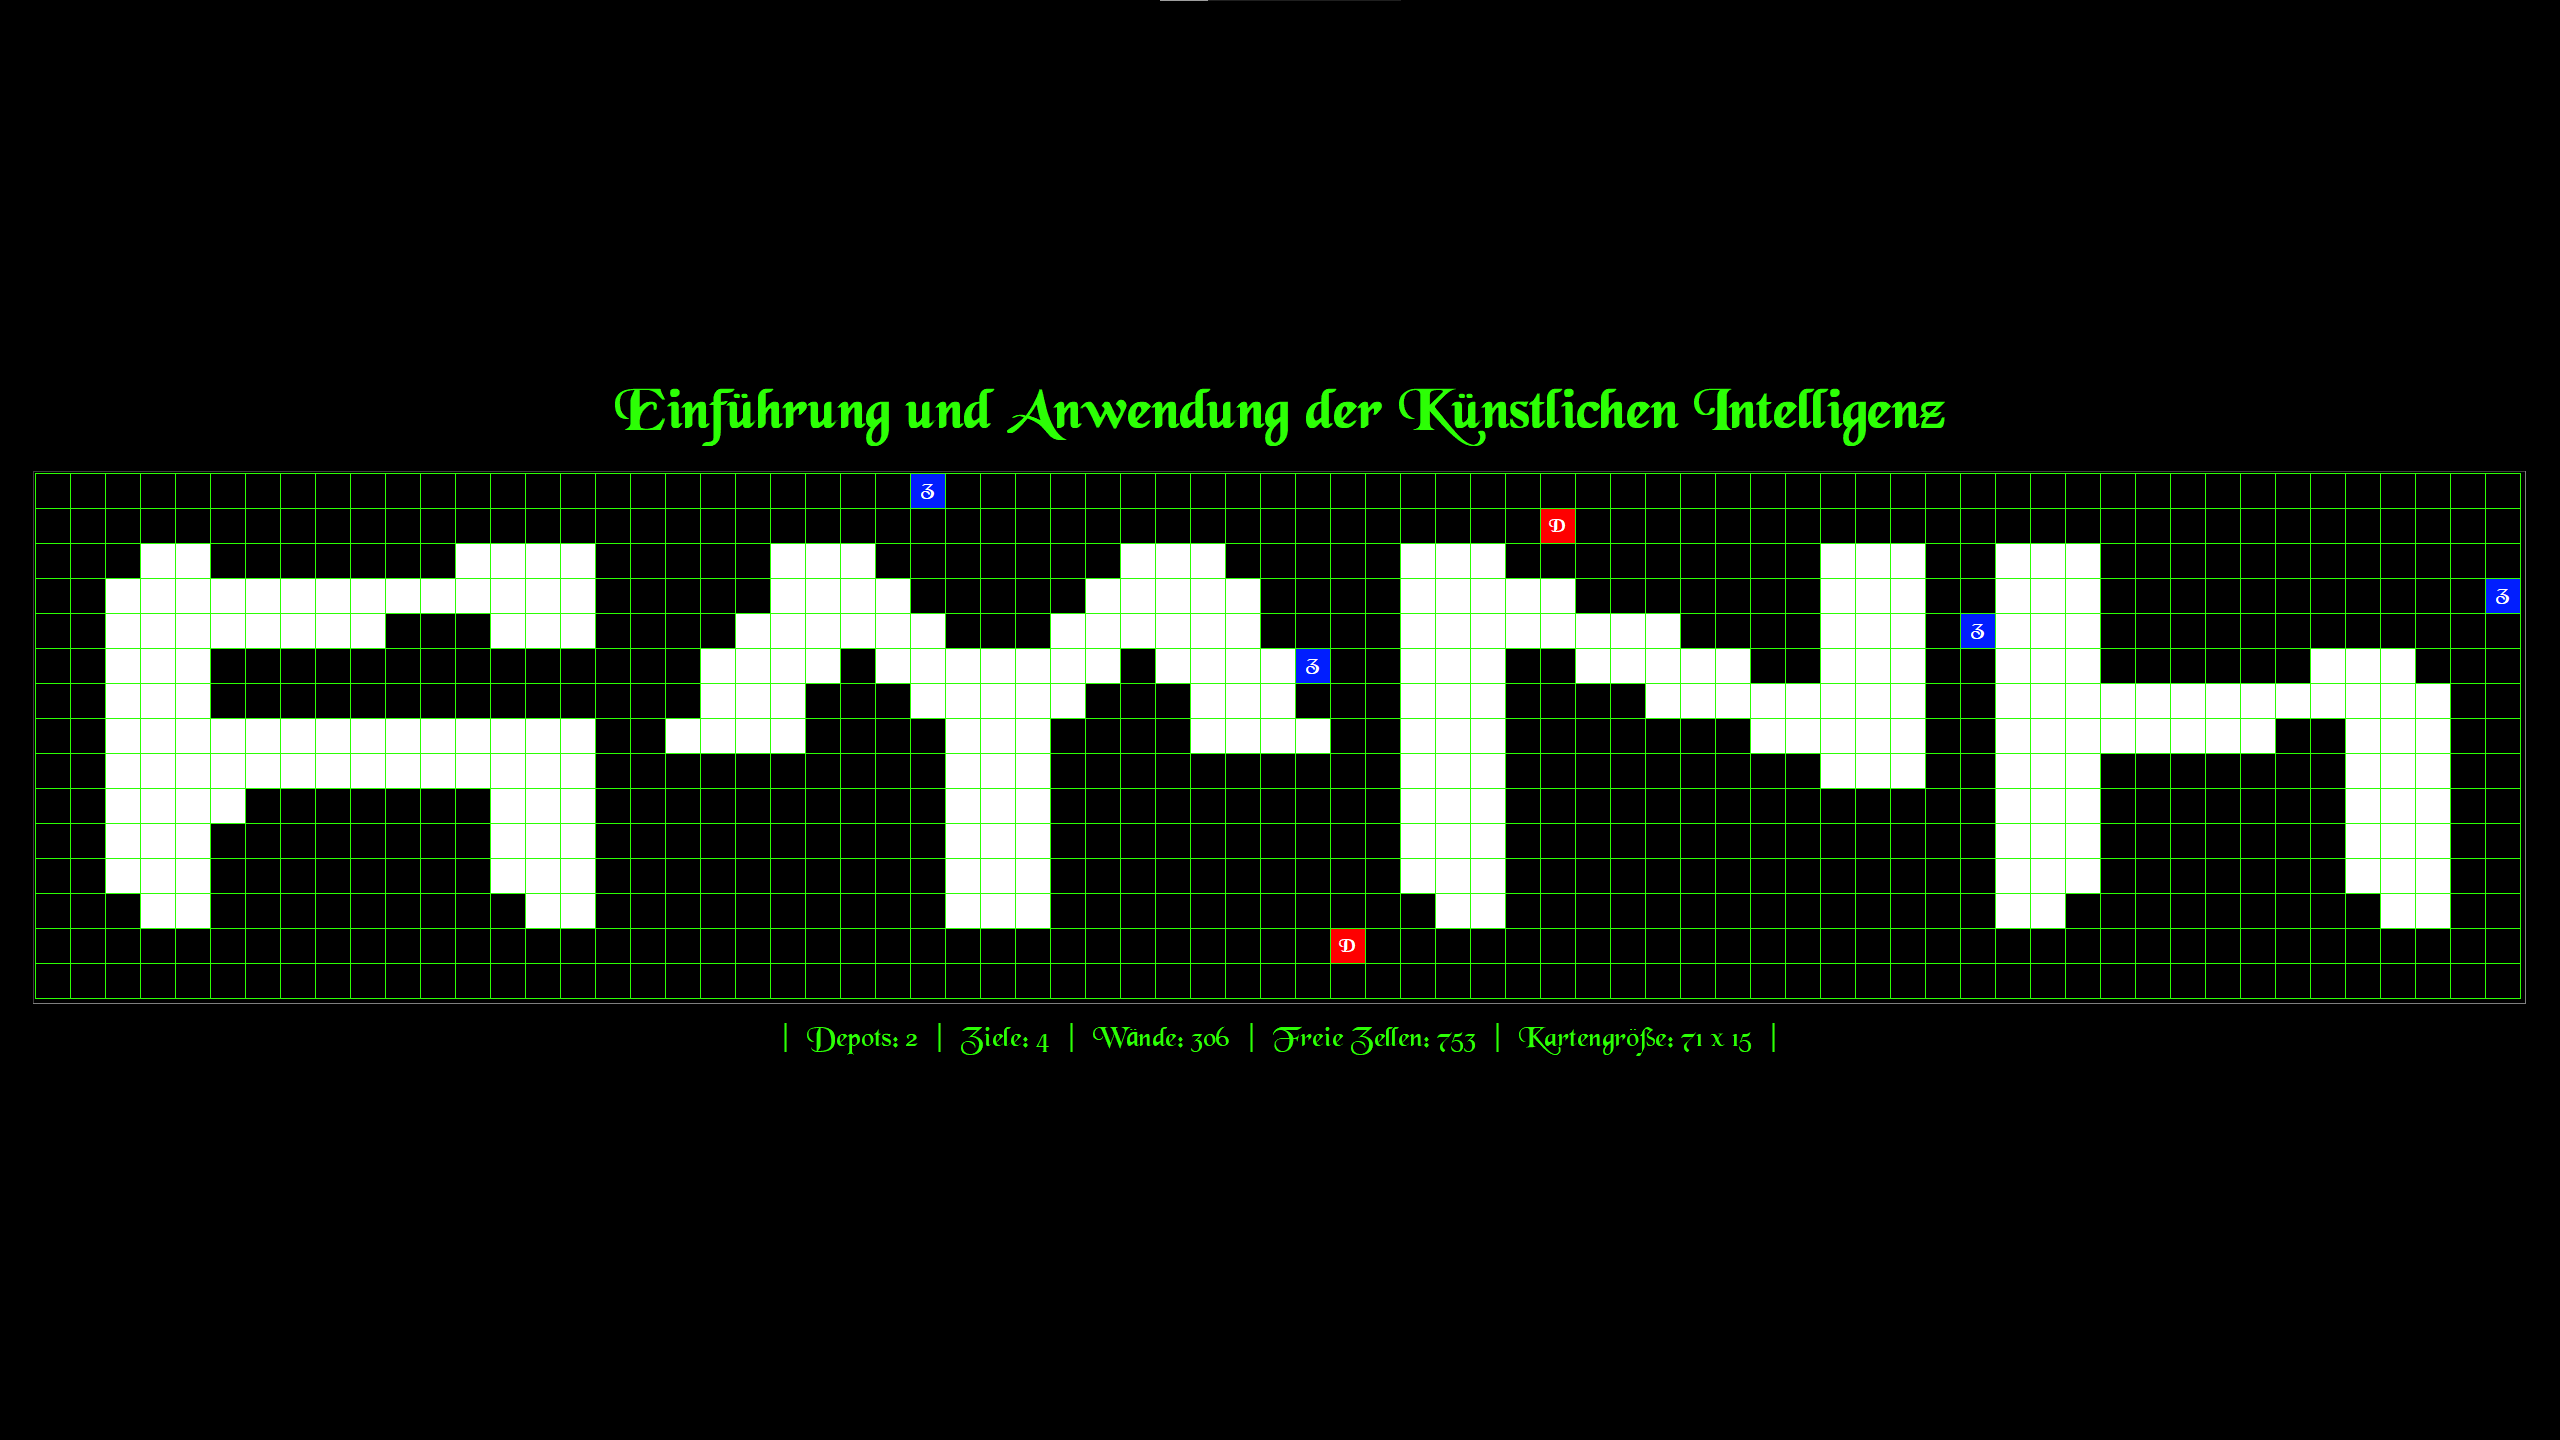
\includegraphics[width=1\textwidth]{asset/image/1A-GUI.png}
    \caption{Grafische Darstellung der Karte in der \acs{GUI} (\acs{D} = Depot, \acs{Z} = Ziel)}
    \label{fig:map1a_gui}
\end{figure}

Die Konsolenausgabe nach der Initialisierung der Karte zeigt die vollständige Karte mit allen Depots und Zielen sowie die zugehörigen Statistiken:

\lstinputlisting[
    style=console,
    caption={Terminal-Ausgabe nach Karteninitialisierung},
    label={lst:map1a_terminal}
]{asset/code/1A-terminal.tex}

Die Ausgabe zeigt:
\begin{itemize}
    \item Die Kartengröße von 71×15 Zellen (inklusive freiem Rand).
    \item Die Positionen der zwei Depots (\acs{D}) und vier Ziele (\acs{Z}) – zufällig, aber reproduzierbar durch den Seed.
    \item Die Anzahl der Wände (306) und freien Zellen (753).
    \item Die Karte selbst, bei der die Wände das \acs{ASCII}-Art-Muster bilden.
\end{itemize}

Die Kartenstatistiken sind in Tabelle \ref{tab:map1a_stats} zusammengefasst.

\begin{table}[H]
    \centering
    \begin{tabular}{l r}
        \toprule
        \textbf{Merkmal} & \textbf{Wert} \\
        \midrule
        Kartengröße & 71×15 Zellen \\
        Depots & 2 \\
        Ziele & 4 \\
        Wände & 306 \\
        Freie Zellen & 753 \\
        \bottomrule
    \end{tabular}
    \caption{Statistiken der Karte}
    \label{tab:map1a_stats}
\end{table}

Die Besonderheit der Karte ist in der \acs{GUI} und der \acs{ASCII}-Repräsentation deutlich erkennbar.

% ==============================================================================
% ========================= Aufgabe 1B - Agentenmodell ========================
% ==============================================================================

\section{Agentenmodell \textit{1b}}
\label{sec:aufgabe1b}

\subsection{Aufgabenstellung}

Implementieren Sie ein Agentenmodell mit Position \((x, y)\), Geschwindigkeit in Zellen pro Simulationsschritt, Kapazität (in Paketeinheiten) und Batteriestand. Erzeugen Sie mindestens zwei Agententypen, Standard und Express.

\subsection{Theoretische Grundlagen}

Gemäß Aufgabenstellung sind die Lieferroboter als \textit{Agenten} im Sinne der Künstlichen Intelligenz zu modellieren. \textcite[S. 7]{5} grenzt den Agentenbegriff wie folgt ab: Während klassische Programme ausschließlich reaktiv auf Eingaben reagieren, \enquote{handelt ein Softwareagent -- oder Agent im Allgemeinen -- \ldots von sich aus, um ein bestimmtes Ziel zu erreichen oder einen Zustand herzustellen. Diese \enquote{Motivation} ist der wesentliche Unterschied}. Formaler definiert \textcite[S. 8]{5}: \enquote{Ein Agent ist eine Entität, die ihre Umgebung durch Sensoren überwacht und sie mittels Aktuatoren verändert.}

Zur systematischen Beschreibung eines Agenten dient das \textit{\acs{PEAS}}-Ordnungsschema (\textit{Performance Measure, Environment, Actuators, Sensors}), das in \textcite[S. 8\,f.]{5} eingeführt wird. Für einen Lieferroboter auf einer diskreten Karte lässt sich die Zuordnung wie folgt vornehmen:

\begin{table}[H]
    \centering
    \begin{tabular}{p{4.5cm} p{9.5cm}}
        \toprule
        \textbf{\acs{PEAS}-Komponente} & \textbf{Lieferroboter} \\
        \midrule
        Performance Measure & Zugestellte Pakete pro Zeitintervall, Energieeffizienz \\
        Environment          & Diskrete 2D-Karte (vgl. Aufgabe 1a) \\
        Actuators            & Bewegung auf Nachbarzellen, Paket aufnehmen/abliefern \\
        Sensors              & Aktuelle Position \((x, y)\), Batteriestand, Ladung \\
        \bottomrule
    \end{tabular}
    \caption{\acs{PEAS}-Klassifikation des Lieferroboters (in Anlehnung an \cite{5})}
    \label{tab:peas_agent_1b}
\end{table}

Die in Aufgabe 1b geforderten Attribute (Position, Geschwindigkeit, Kapazität, Batteriestand) bilden damit die \textit{Zustandsgrößen} des Agenten, die zur Laufzeit durch Sensoren erfasst bzw. durch Aktuatoren verändert werden. Da der Agent diese internen Zustandsinformationen speichert und zur Handlungsgrundlage heranzieht, ist er als \textit{modellbasierter Agent} im Sinne von \textcite[S. 18\,f.]{5} einzuordnen.

\subsection{Implementierung}

Das Agentenmodell wird in einem eigenen Modul \texttt{agent.py} realisiert, das nach dem in der Einleitung eingeführten Architekturprinzip der \textit{Separation of Concerns} (vgl. Abschnitt~\ref{chap:einleitung}) ausschließlich die Fachlogik der Agenten enthält. Die Konfiguration folgt dem \textit{Single-Source-of-Truth}-Prinzip: Sämtliche Werte -- Typen, Geschwindigkeiten, Kapazitäten, Batteriestände, Symbole, Farben, Log-Texte und Fehlermeldungen -- sind zentral in \texttt{config.py} im Block \texttt{AUFGABE 1B} definiert. Im Modul \texttt{agent.py} existiert dadurch keine Hardcodierung.

% ======= config.py – Block 1B: Agenten-Konfiguration =======

\subsubsection{Konfiguration \texttt{config.py} – Agentenparameter}

Der neue Konfigurationsblock definiert alle agentenspezifischen Werte:

\lstinputlisting[
    language=python,
    style=python,
    caption={Agentenspezifische Konfiguration (\texttt{config.py})},
    label={lst:config_agent},
    firstline=140,
    lastline=189
]{asset/code/1B-config.py}

Diese Konfiguration umfasst:
\begin{itemize}
    \item \texttt{TomaKing1B\_TypeStandard} und \texttt{TomaKing1B\_TypeExpress} – Die beiden Agententypen.
    \item \texttt{TomaKing1B\_StartAgentId} – Startwert für die fortlaufende ID-Vergabe.
    \item \texttt{TomaKing1B\_CountStandard}, \texttt{TomaKing1B\_CountExpress} – Anzahl der zu erzeugenden Agenten je Typ.
    \item \texttt{TomaKing1B\_Seed} – Seed für reproduzierbare Platzierung (verweist auf \texttt{TomaKing1A\_Seed}, um die Reproduzierbarkeit über beide Aufgaben hinweg konsistent zu halten).
    \item \texttt{TomaKing1B\_SpeedStandard} (1) und \texttt{TomaKing1B\_SpeedExpress} (2) – Geschwindigkeit in Zellen pro Simulationsschritt.
    \item \texttt{TomaKing1B\_CapacityStandard} (5) und \texttt{TomaKing1B\_CapacityExpress} (3) – Kapazität in Paketeinheiten.
    \item \texttt{TomaKing1B\_InitialCargo} – Anfangsladung (0).
    \item \texttt{TomaKing1B\_BatteryStandard} (100) und \texttt{TomaKing1B\_BatteryExpress} (120) – Startbatteriestand.
    \item \texttt{TomaKing1B\_SymbolStandard} (\texttt{"S"}) und \texttt{TomaKing1B\_SymbolExpress} (\texttt{"E"}) – Kürzel für die \acs{GUI}-Zeichnung.
    \item \texttt{TomaKing1B\_ColorStandard}, \texttt{TomaKing1B\_ColorExpress}, \texttt{TomaKing1B\_RadiusFactor} – Farben und Größe der Agentenkreise.
    \item \texttt{TomaKing1B\_LabelAgents}, \texttt{TomaKing1B\_LabelStandard}, \texttt{TomaKing1B\_LabelExpress}, \texttt{TomaKing1B\_LabelAgentParts} – Beschriftungen der Info-Zeile.
    \item \texttt{TomaKing1B\_StatKey*} – Symbolische Schlüssel des Statistik-Dictionaries für die \acs{GUI} (siehe Abschnitt~\ref{sssec:agent_stats}).
    \item \texttt{TomaKing1B\_ReprTemplate} – Template für die \texttt{\_\_repr\_\_}-Ausgabe.
    \item \texttt{TomaKing1B\_LogColumnFormat}, \texttt{TomaKing1B\_LogAgentsHeaderLabels}, \\ \texttt{TomaKing1B\_LogAgentPosition}, \texttt{TomaKing1B\_LogAgentBattery} – Formatdefinitionen für das Konsolen-Logging.
    \item \texttt{TomaKing1B\_ErrorUnknownType}, \texttt{TomaKing1B\_ErrorNotEnoughCellsForAgents} – Fehlermeldungen für unbekannte Typen und zu wenige freie Zellen.
\end{itemize}

Die Validierungsliste in \texttt{validate\_config()} wird entsprechend erweitert. Auch die neuen Konstanten werden beim Import geprüft, sodass ein fehlender Wert sofort mit einer präzisen Fehlermeldung abbricht (vgl. Abschnitt~\ref{sssec:config_validierung}).

% ======= agent.py – Block 1: Imports und Agent-Klasse =======

\subsubsection{Modul \texttt{agent.py} – Imports und Agent-Klasse}

Das Modul \texttt{agent.py} implementiert das Agentenmodell. Der erste Block enthält die Importe und die Klassendefinition:

\lstinputlisting[
    language=python,
    style=python,
    caption={Imports und Agent-Klasse (\texttt{agent.py})},
    label={lst:agent_imports},
    firstline=5,
    lastline=92
]{asset/code/1B-agent.py}

Die Klasse \texttt{Agent} kapselt den vollständigen Zustand eines Lieferroboters. Der Konstruktor:
\begin{itemize}
    \item setzt die übergebene Agenten-ID, den Typ und die Startposition \((x, y)\),
    \item lädt die typabhängigen Attributwerte (Geschwindigkeit, Kapazität, Batteriestand) aus der zentralen Konfiguration,
    \item speichert den initialen Batteriestand zusätzlich als \texttt{battery\_max}, damit spätere Prozentberechnungen einen Referenzwert haben,
    \item initialisiert die Ladung (\texttt{cargo}) mit dem konfigurierten Anfangswert.
\end{itemize}

Für die Typ-Differenzierung wird eine explizite \texttt{if/elif}-Verzweigung verwendet. Da die Aufgabenstellung ausschließlich die zwei Typen \textit{Standard} und \textit{Express} vorsieht, ist diese Lösung hinreichend. Bei einem unbekannten Typ löst der Konstruktor eine \texttt{ValueError}-Ausnahme mit der konfigurierten Fehlermeldung aus, sodass eine stille Fehlklassifikation ausgeschlossen wird.

Neben dem Konstruktor stellt die Klasse drei öffentliche Methoden bereit:
\begin{itemize}
    \item \texttt{get\_position()} – Liefert die aktuelle Position als Tupel \texttt{(x, y)}. Grundlage für die \acs{GUI}-Zeichnung und spätere Navigationsoperationen (\acs{Astern}, Aufgabe 3).
    \item \texttt{to\_string()} – Erzeugt eine tabellarisch formatierte Zeile mit allen Attributen (ID, Typ, Position, Speed, Kapazität, Batterie, Ladung). Das Format ist vollständig in \texttt{TomaKing1B\_LogColumnFormat} definiert.
    \item \texttt{\_\_str\_\_()} und \texttt{\_\_repr\_\_()} – Werden von \texttt{print()} bzw. zur Debug-Ausgabe verwendet. Die Repräsentation nutzt das konfigurierte Template \\ \texttt{TomaKing1B\_ReprTemplate}.
\end{itemize}

% ======= agent.py – Block 2: Agent-Fabrik =======

\subsubsection{Modul \texttt{agent.py} – Agent-Fabrik}

Die Funktion \texttt{create\_agents} erzeugt alle Agenten an zufälligen, aber reproduzierbaren Positionen. Mit der Erzeugung mehrerer gleichzeitig existierender Agenten wird damit der Übergang vom Einzelagenten zum \textit{Multiagentensystem} vollzogen -- einer Gruppe von Agenten, die eine gemeinsame Problemstellung bearbeiten \cite[S. 29\,f.]{5}:

\lstinputlisting[
    language=python,
    style=python,
    caption={Agent-Fabrik (\texttt{agent.py})},
    label={lst:agent_factory},
    firstline=94,
    lastline=115
]{asset/code/1B-agent.py}

Der Ablauf ist wie folgt:
\begin{enumerate}
    \item Ermittlung der Gesamtzahl der zu erzeugenden Agenten aus den beiden Konfigurationswerten.
    \item Abfrage aller freien Zellen über die neue öffentliche Methode \texttt{map.get\_free\_cells()} (vgl. Abschnitt~\ref{sssec:map_get_free_cells}).
    \item Prüfung, ob ausreichend freie Zellen vorhanden sind. Andernfalls wird die konfigurierte Fehlermeldung ausgegeben.
    \item Setzen des Seeds (\texttt{TomaKing1B\_Seed}) und Auswahl von \texttt{total} unterschiedlichen freien Zellen über \texttt{random.sample}. Der Seed gewährleistet, dass die Positionen bei jedem Programmaufruf identisch sind -- dies ist für die Reproduzierbarkeit der späteren Simulationsergebnisse (Aufgabe 5) essenziell.
    \item Erzeugung der Standard-Agenten (erste \texttt{CountStandard} Zellen), anschließend der Express-Agenten.
    \item Fortlaufende ID-Vergabe, beginnend bei \texttt{TomaKing1B\_StartAgentId}.
    \item Aufruf der Logging-Funktion \texttt{\_log\_agents}, die die Agenten einmalig bei Erzeugung auf der Konsole protokolliert.
\end{enumerate}

Die Agenten werden bewusst \textbf{nicht} in die Karten-Datenstruktur \texttt{Map.\_data} eingetragen, sondern ausschließlich in eigenen Objekten gehalten. Damit bleibt das Kartenmodell unverändert, und die Agenten können sich in späteren Aufgaben (1c, 3) unabhängig von der statischen Karte bewegen.

% ======= agent.py – Block 3: Statistiken und Logging =======

\subsubsection{Modul \texttt{agent.py} – Statistiken und Logging}
\label{sssec:agent_stats}

Die Funktionen für Statistiken und Logging erfassen die Agenten-Kennzahlen und protokollieren sie:

\lstinputlisting[
    language=python,
    style=python,
    caption={Statistiken und Logging (\texttt{agent.py})},
    label={lst:agent_stats},
    firstline=117,
    lastline=138
]{asset/code/1B-agent.py}

\texttt{get\_agent\_statistics} liefert ein Dictionary mit den Kennzahlen für die \acs{GUI}-Info-Zeile -- Gesamtzahl, Anzahl Standard, Anzahl Express -- sowie der Agentenliste selbst. Die Schlüssel des Dictionaries sind nicht als Zeichenketten im Code verankert, sondern ausschließlich als symbolische Konstanten (\texttt{TomaKing1B\_StatKey*}) definiert. Dadurch sind die Schlüssel in \texttt{agent.py} (schreibender Zugriff) und \texttt{gui.py} (lesender Zugriff) gegen Tippfehler abgesichert.

\texttt{\_log\_agents} gibt die vollständige Agentenliste einmalig bei der Erzeugung auf der Konsole aus. Die Ausgabe verwendet das konfigurierte Spaltenformat und die konfigurierten Trennzeichen. Die Log-Ausgabe dient als Ergebnisnachweis (vgl. Abschnitt~\ref{sssec:agent_ergebnisnachweis}).

% ======= map.py – Erweiterung get_free_cells =======

\subsubsection{Modul \texttt{map.py} – Erweiterung \texttt{get\_free\_cells}}
\label{sssec:map_get_free_cells}

Damit die Agenten-Fabrik auf die freien Zellen der Karte zugreifen kann, wird die Klasse \texttt{Map} um eine öffentliche Methode erweitert:

\lstinputlisting[
    language=python,
    style=python,
    caption={Erweiterung \texttt{get\_free\_cells} (\texttt{map.py})},
    label={lst:map_freecells},
    firstline=166,
    lastline=173
]{asset/code/1B-map.py}

Die Methode iteriert über alle Zellen der Karte und sammelt die Positionen ein, deren Wert dem konfigurierten Symbol für freie Zellen (\texttt{TomaKing1A\_Empty}) entspricht. Sie ist damit konsistent mit der bereits in \texttt{\_place\_depots\_and\_targets} verwendeten Logik und nutzt ausschließlich die zentrale Konfiguration. Es existiert keine Hardcodierung.

% ======= gui.py – Block 1: Erweiterte Imports =======

\subsubsection{Modul \texttt{gui.py} – Erweiterte Imports}

Für die Darstellung der Agenten werden die Symbole, Farben und Statistik-Schlüssel aus dem 1B-Block importiert:

\lstinputlisting[
    language=python,
    style=python,
    caption={Erweiterte Imports (\texttt{gui.py})},
    label={lst:gui_imports_1b},
    firstline=95,
    lastline=112
]{asset/code/1B-gui.py}

Und der Import aus \texttt{agent} der \texttt{create\_agents} und \texttt{get\_agent\_statistics} elemente:

\lstinputlisting[
    language=python,
    style=python,
    caption={agent Imports (\texttt{gui.py})},
    label={lst:gui_agent_imports_1b},
    firstline=11,
    lastline=11
]{asset/code/1B-gui.py}

% ======= gui.py – Block 2: Konstruktor-Erweiterung =======

\subsubsection{Modul \texttt{gui.py} – Konstruktor-Erweiterung}

Der Konstruktor von \texttt{Map\acs{GUI}} wird um die Erzeugung der Agenten ergänzt:

\lstinputlisting[
    language=python,
    style=python,
    caption={Konstruktor-Erweiterung (\texttt{gui.py})},
    label={lst:gui_ctor_1b},
    firstline=129,
    lastline=129
]{asset/code/1B-gui.py}

Nach dem Aufbau der Karte (\texttt{self.map = Map()}) werden die Agenten über \\ \texttt{create\_agents(self.map)} erzeugt und in \texttt{self.agents} gespeichert. Der Seed stellt sicher, dass die Platzierung reproduzierbar ist.

% ======= gui.py – Block 3: Erweiterte Info-Zeile =======

\subsubsection{Modul \texttt{gui.py} – Erweiterte Info-Zeile}

Die Info-Zeile wird um eine Agenten-Sektion ergänzt:

\lstinputlisting[
    language=python,
    style=python,
    caption={Erweiterte Info-Zeile (\texttt{gui.py})},
    label={lst:gui_info_1b},
    firstline=218,
    lastline=226
]{asset/code/1B-gui.py}

Die Darstellung folgt dem bereits in 1a eingeführten Muster: Die Agenten-Statistiken werden aus \texttt{get\_agent\_statistics(self.agents)} bezogen und mit den konfigurierten Beschriftungen und Separatoren an die Karten-Statistiken angehängt. 

\paragraph{Hinweis zum späteren Refactoring.}
Der 1B-Block der Info-Zeile wurde in Aufgabe 1c in die Methode \texttt{\_build\_info\_text} überführt (siehe Abschnitt~\ref{sssec:refactoring_info_1c}).

% ======= gui.py – Block 4: Agenten zeichnen =======

\subsubsection{Modul \texttt{gui.py} – Agenten zeichnen}

Die Methode \texttt{\_draw\_agents} zeichnet alle Agenten als farbige Kreise mit Typ-Symbol:

\lstinputlisting[
    language=python,
    style=python,
    caption={Agenten zeichnen (\texttt{gui.py})},
    label={lst:gui_draw_agents},
    firstline=288,
    lastline=323
]{asset/code/1B-gui.py}

Die Methode wird am Ende von \texttt{\_draw\_map} aufgerufen, sodass die Agenten stets über der Karte gezeichnet werden. Für jeden Agenten:
\begin{itemize}
    \item wird die aktuelle Position über \texttt{agent.get\_position()} ermittelt,
    \item der Mittelpunkt der zugehörigen Zelle berechnet,
    \item der Radius aus Zellgröße und \texttt{TomaKing1B\_RadiusFactor} bestimmt,
    \item die Farbe (Orange für Standard, Gelb für Express) und das Symbol (\texttt{S} bzw. \texttt{E}) aus der Konfiguration gewählt,
    \item ein gefüllter Kreis (\texttt{create\_oval}) mit weißer Umrandung gezeichnet,
    \item das Typ-Symbol mittig in weißer Farbe eingefügt.
\end{itemize}

Da \texttt{\_draw\_map} sowohl beim Initialaufbau als auch bei jeder Fenstergrößenänderung aufgerufen wird (vgl. Abschnitt~1.1.3.11 in Aufgabe 1a), werden die Agenten bei jeder Größenänderung automatisch neu skaliert.

% ======= gui.py – Anbindung in _draw_map =======

\subsubsection{Modul \texttt{gui.py} – Anbindung in \texttt{\_draw\_map}}

Der Aufruf der Agenten-Zeichnung erfolgt am Ende der bestehenden Methode \texttt{\_draw\_map} aus Aufgabe 1a:

\lstinputlisting[
    language=python,
    style=python,
    caption={Aufruf von \texttt{\_draw\_agents} in \texttt{\_draw\_map} (\texttt{gui.py})},
    label={lst:gui_draw_call_1b},
    firstline=286,
    lastline=286
]{asset/code/1B-gui.py}

Die Platzierung am Ende von \texttt{\_draw\_map} ist bewusst gewählt:
\begin{enumerate}
    \item \texttt{\_draw\_map} wird sowohl beim Initialaufbau (in \texttt{\_create\_widgets}) als auch bei jeder Fenstergrößenänderung (in \texttt{\_update\_layout}) aufgerufen. Durch die Bündelung bleibt die Aufrufkette unverändert, und die Agenten werden bei jeder Skalierung automatisch neu gezeichnet.
    \item Da Canvas-Elemente in der Reihenfolge ihres Anlegens übereinander liegen, müssen die Agentenkreise \textit{nach} den Kartenzellen gezeichnet werden. Andernfalls würden sie von den Zellrechtecken überdeckt.
    \item Die Trennung der beiden Zeichenmethoden bleibt erhalten: \texttt{\_draw\_map} ist für die Karte, \texttt{\_draw\_agents} für die Agenten zuständig. Dies entspricht dem Prinzip der \textit{Separation of Concerns} auf Methodenebene (vgl. Abschnitt~\ref{chap:einleitung}).
\end{enumerate}

Der Aufruf erfolgt ohne Parameter -- die Agentenliste ist über \texttt{self.agents} im \acs{GUI}-Objekt verfügbar und wird vom Konstruktor befüllt (vgl. Abschnitt~\ref{sec:aufgabe1b}). Es existiert keine Hardcodierung: Der Aufruf referenziert ausschließlich die Methode \texttt{\_draw\_agents}, deren Farb-, Symbol- und Größenwerte vollständig aus \texttt{config.py} bezogen werden.

% ======= Ergebnisnachweis =======

\subsection{Ergebnisnachweis}
\label{sssec:agent_ergebnisnachweis}

Abbildung~\ref{fig:agent1b_gui} zeigt die grafische Darstellung der Karte mit den Agenten in der \acs{GUI}. Die Agenten sind als farbige Kreise mit den Typ-Kürzeln \texttt{\acs{S}} (Standard) und \texttt{\acs{E}} (Express) an ihren Positionen dargestellt. Die Info-Zeile unterhalb der Karte enthält zusätzlich die Agenten-Zählung.

\begin{figure}[H]
    \centering
    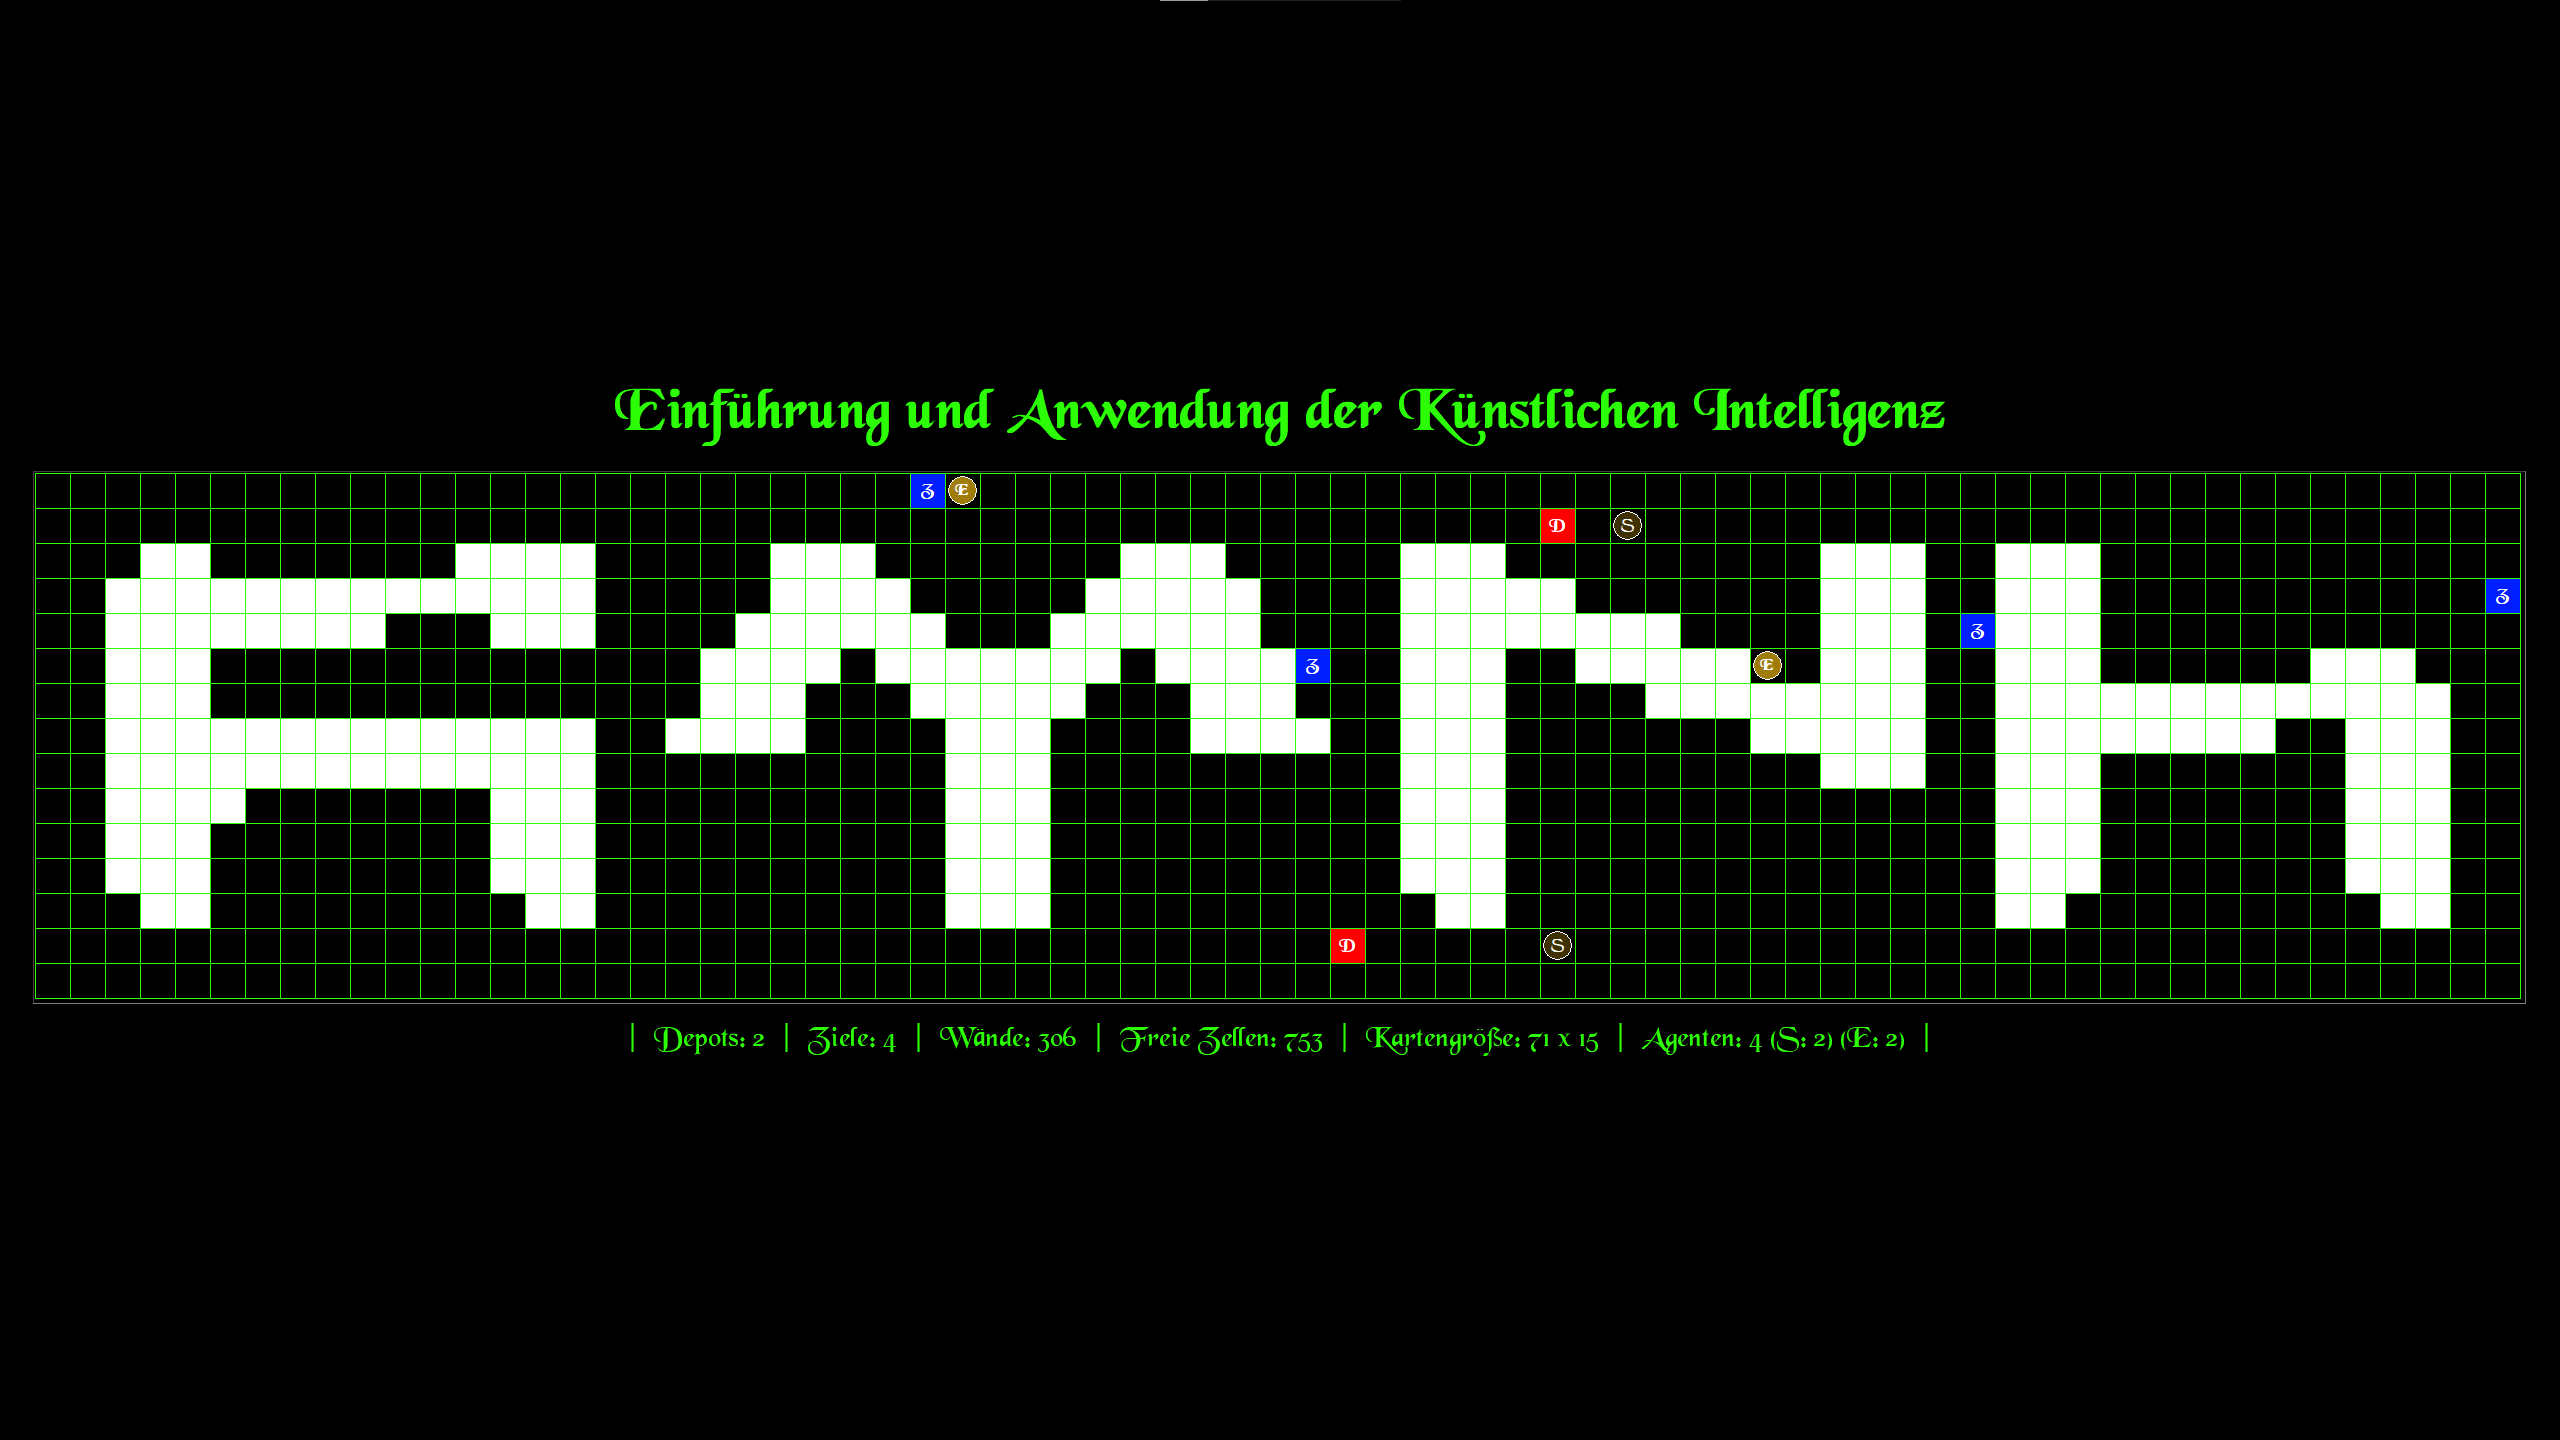
\includegraphics[width=1\textwidth]{asset/image/1B-GUI.png}
    \caption{Grafische Darstellung der Karte mit Agenten (\acs{S}, \acs{E})}
    \label{fig:agent1b_gui}
\end{figure}

Nach dem Start der Anwendung werden auf der Konsole zunächst die Kartendaten (aus Aufgabe 1a) und anschließend die Agenten protokolliert:

\lstinputlisting[
    style=console,
    caption={Terminal-Ausgabe: Agenten nach der Erzeugung},
    label={lst:agent1b_terminal}
    firstline=24,
    lastline=31
]{asset/code/1B-gui.py}

Die Ausgabe zeigt:
\begin{itemize}
    \item Die Tabelle wird durch je eine Trennlinie (konfiguriert über \\ \texttt{TomaKingGUI\_LogSeparatorCharEqual} und \texttt{TomaKingGUI\_LogSeparatorCharLine}) eingerahmt.
    \item Die Kopfzeile enthält die Spaltenüberschriften aus \texttt{TomaKing1B\_LogAgentsHeaderLabels}.
    \item Es werden vier Agenten aufgelistet -- zwei Standard und zwei Express -- mit fortlaufenden IDs.
    \item Die Express-Agenten haben Speed 2, Kapazität 3 und Batterie 120, die Standard-Agenten Speed 1, Kapazität 5 und Batterie 100.
    \item Die Ladung ist bei allen Agenten mit 0 initialisiert.
    \item Die Positionen sind zufällig, aber durch den Seed reproduzierbar.
\end{itemize}

Die Agenteneigenschaften sind in Tabelle~\ref{tab:agent1b_properties} zusammengefasst.

\begin{table}[H]
    \centering
    \begin{tabular}{l r r}
        \toprule
        \textbf{Eigenschaft} & \textbf{Standard} & \textbf{Express} \\
        \midrule
        Geschwindigkeit (Zellen/Schritt) & 1 & 2 \\
        Kapazität (Paketeinheiten)       & 5 & 3 \\
        Batteriestand                    & 100 & 120 \\
        Anzahl                           & 2 & 2 \\
        \bottomrule
    \end{tabular}
    \caption{Eigenschaften der Agententypen}
    \label{tab:agent1b_properties}
\end{table}

% ==============================================================================
% ================= Aufgabe 1C - Simulation und Hauptschleife =================
% ==============================================================================

\section{Simulation und Hauptschleife \textit{1c}}
\label{sec:aufgabe1c}

\subsection{Aufgabenstellung}

Implementieren Sie die Initialisierung und Hauptschleife der Simulation. Pro Schritt können Agenten Nachrichten empfangen/lesen, Handlungen planen und eine Handlung ausführen (Bewegung, Paket aufnehmen, Paket abliefern, Nachricht senden). Für die Bewegungslogik können Sie zunächst zum Testen eine zufällige Richtungswahl implementieren; die eigentliche Wegplanung ist Gegenstand von Aufgabe 3.

\subsection{Theoretische Grundlagen}

Mit der Einführung einer Hauptschleife, die Agenten zyklisch Nachrichten lesen, planen und handeln lässt, wird der Übergang von einem einzelnen, statischen Agentenmodell (Aufgabe 1b) zu einem \textit{Multiagentensystem} vollzogen. \textcite[S. 29\,f.]{5} definiert: \enquote{Wenn mehrere Agenten miteinander interagieren und dabei eine gemeinsame Problemstellung bearbeiten, spricht man von einem \textit{Multiagentensystem (MAS)}. Das Verhalten der Agenten zueinander wird dabei von ihrem gemeinsamen Kommunikationsprotokoll, also einer Menge an Verhaltensregeln, bestimmt.} Die in 1c eingeführte Nachrichten-Infrastruktur (Message-Klasse und Nachrichten-Bus) ist damit die technische Vorbereitung für das in Aufgabe 2 folgende \textit{Contract-Net-Protokoll}. Der schrittweise Ablauf der Hauptschleife entspricht dabei dem Konzept eines \textit{diskreten Zeitsystems}: Die Simulation unterteilt die Zeit in feste Schritte, in denen alle Agenten genau eine Handlung ausführen können \cite[S. 13]{5}.

Die vier in der Aufgabenstellung genannten Handlungstypen (Bewegung, Aufnehmen, Abliefern, Senden) entsprechen den in \textcite[S. 8]{5} definierten \textit{Aktuatoren} eines Agenten -- also den Komponenten, mit denen der Agent auf seine Umgebung einwirkt. Das Nachrichten-Lesen entspricht der \textit{Sensor}-Seite. In \textcite[S. 14\,ff.]{5} wird eine solche Architektur als \textit{reflexbasierter Agent} beschrieben: Der Agent wählt seine Aktion ausschließlich auf Basis seiner aktuellen Wahrnehmung und eines festen Regelsatzes.

Da unser Agent zusätzlich seinen internen Zustand (Position, Batterie, Ladung) speichert und daraus seine nächste Aktion ableitet, entspricht er bereits dem erweiterten Modell des \textit{modellbasierten Agenten} \cite[S. 19\,f.]{5}. Der Nachrichten-Austausch zwischen den Agenten folgt dabei bereits dem in Aufgabe 2 formalisierten \textit{Task Announcement Schema} des Contract Net Protocol, das in \textcite[S. 30]{5} beschrieben wird.

Der in der Aufgabenstellung geforderte Testcharakter der Bewegungslogik (zufällige Richtungswahl) ist in \textcite[S. 11]{5} als legitimer Zwischenschritt beschrieben: \enquote{Rationale Agenten können aber auch vollkommen stochastisch handeln, um aus Situationen zu entkommen, in denen sie feststecken.} In Aufgabe 3 wird diese Zufallsstrategie durch die \acs{Astern}-Pfadplanung ersetzt.

\subsection{Implementierung}

Die Simulation wird in einem neuen Modul \texttt{simulation.py} realisiert. Zusätzlich werden zwei Domänenobjekte in eigenen Modulen gekapselt: \texttt{message.py} (Nachrichten-Hülle) und \texttt{package.py} (Paket-Modell). Die Konfiguration folgt weiterhin dem \textit{Single-Source-of-Truth}-Prinzip: Alle Simulationsparameter (Zeitsteuerung, Batterieverbrauch, Button-Layout, Farben, Log-Templates, Fehlermeldungen) sind zentral im Block \texttt{AUFGABE 1C} in \texttt{config.py} definiert. Im Modul \texttt{simulation.py} und in den erweiterten Modulen \texttt{agent.py} und \texttt{gui.py} existiert keine Hardcodierung.

% ======= config.py – Block 1C: Simulations-Konfiguration =======

\subsubsection{Konfiguration \texttt{config.py} – Simulationsparameter}

Der neue Konfigurationsblock definiert alle simulationsspezifischen Werte:

\lstinputlisting[
    language=python,
    style=python,
    caption={Simulationsspezifische Konfiguration (\texttt{config.py})},
    label={lst:config_simulation},
    firstline=191,
    lastline=232
]{asset/code/1C-config.py}

Diese Konfiguration umfasst:
\begin{itemize}
    \item \texttt{TomaKing1C\_Seed} – Seed für die Reproduzierbarkeit. Er verweist auf \texttt{TomaKing1A\_Seed}, um die Konsistenz über alle Aufgaben hinweg zu wahren.
    \item \texttt{TomaKing1C\_StepDelay} – Verzögerung zwischen zwei Schritten im AutoRun-Modus (100\,ms).
    \item \texttt{TomaKing1C\_BatteryMoveBase} (1) und \texttt{TomaKing1C\_BatteryStandstill} (0) – Batterieverbrauch pro ausgeführter Bewegung bzw. pro Stillstand.
    \item \texttt{TomaKing1C\_LogStepHeaderTemplate} – Format-String für die Step-Überschrift.
    \item \texttt{TomaKing1C\_ButtonStepText}, \texttt{\_ButtonAutoRunText}, \texttt{\_ButtonStopText} – Beschriftungen der Steuer-Buttons.
    \item \texttt{TomaKing1C\_ButtonFramePady}, \texttt{\_ButtonPaddingX}, \texttt{\_ButtonFont}, \texttt{\_ButtonFontSize} – Layout-Parameter der Button-Leiste.
    \item \texttt{TomaKing1C\_ColorButton*} – Farben der Buttons in verschiedenen Zuständen (inaktiv, aktiv, hover, disabled).
    \item \texttt{TomaKing1C\_MessageInterval} (5) und \texttt{TomaKing1C\_MessageTypeTest} (\texttt{"TEST"}) – Intervall und Typ der automatisch generierten Testnachrichten.
    \item \texttt{TomaKing1C\_LabelStep} und \texttt{TomaKing1C\_StatKeyStepCount} – Beschriftung und Statistik-Schlüssel für die Step-Anzeige in der Info-Zeile.
    \item \texttt{TomaKing1C\_LogSendTemplate}, \texttt{\_LogReadTemplate}, \\ \texttt{\_LogPickUpTemplate}, \texttt{\_LogDeliverTemplate} – Format-Strings für die vier Handlungsprotokolle.
    \item \texttt{TomaKing1C\_ErrorInvalidMessage} – Fehlermeldung für eine Nachricht an einen nicht existierenden Empfänger.
\end{itemize}

Die Validierungsliste in \texttt{validate\_config()} wird um alle neuen Konstanten erweitert (vgl. Abschnitt~\ref{sssec:config_validierung}).

% ======= message.py =======

\subsubsection{Modul \texttt{message.py} – Nachrichten-Infrastruktur}

Die Klasse \texttt{Message} kapselt eine Nachricht zwischen zwei Agenten:

\lstinputlisting[
    language=python,
    style=python,
    caption={Message-Klasse (\texttt{message.py})},
    label={lst:message_class},
    firstline=5,
    lastline=19
]{asset/code/1C-message.py}

Die Attribute sind bewusst minimal gehalten:
\begin{itemize}
    \item \texttt{sender\_id} – ID des sendenden Agenten.
    \item \texttt{receiver\_id} – ID des empfangenden Agenten.
    \item \texttt{msg\_type} – Typ der Nachricht (in 1c nur \texttt{"TEST"}; ab Aufgabe 2 folgen \texttt{ANNOUNCE}, \texttt{BID}, \texttt{AWARD}).
    \item \texttt{payload} – optionale Nutzlast für spätere Nachrichteninhalte.
\end{itemize}

Die Repräsentation über \texttt{\_\_repr\_\_} dient dem Debugging und vermeidet eine zirkuläre Abhängigkeit zur Log-Formatierung.

% ======= package.py =======

\subsubsection{Modul \texttt{package.py} – Paket-Domänenobjekt}

Die Klasse \texttt{Package} bereitet das in Aufgabe 2 einzuführende Paketmodell vor:

\lstinputlisting[
    language=python,
    style=python,
    caption={Package-Klasse (\texttt{package.py})},
    label={lst:package_class},
    firstline=5,
    lastline=23
]{asset/code/1C-package.py}

Das Attribut \texttt{size} (Standard 1) kapselt die Kapazitätseinheit eines Pakets. Es wird in \texttt{Agent.pick\_up} und \texttt{Agent.deliver} verwendet, um die Ladungsänderung semantisch korrekt abzubilden -- anstatt einer hartkodierten Konstante. Pakete werden in 1c noch nicht erzeugt, die Klasse ist reine Infrastruktur so wie aufgefordert.

% ======= simulation.py – Simulation-Klasse =======

\subsubsection{Modul \texttt{simulation.py} – Simulations-Klasse}

Die Klasse \texttt{Simulation} hält Karte, Agentenliste, Nachrichten-Bus und Step-Zähler:

\lstinputlisting[
    language=python,
    style=python,
    caption={Simulations-Klasse (\texttt{simulation.py})},
    label={lst:simulation_class},
    firstline=5,
    lastline=41
]{asset/code/1C-simulation.py}

Der Konstruktor initialisiert den Nachrichten-Bus und setzt den Step-Zähler auf 0. Der Seed wird aus der Konfiguration übernommen, um reproduzierbare zufällige Bewegungen zu gewährleisten.

Die Methode \texttt{log\_event} puffert Events (Nachrichten, später Auktionen) und gibt sie im nächsten Step-Log aus. Damit ist die Ausgabereihenfolge unabhängig von der Reihenfolge der Methodenaufrufe innerhalb der Agentenschleife.

% ======= simulation.py – Nachrichten-Bus =======

\subsubsection{Modul \texttt{simulation.py} – Nachrichten-Bus}

Der Nachrichten-Bus ist als einfache Liste implementiert:

\lstinputlisting[
    language=python,
    style=python,
    caption={Nachrichten-Bus (\texttt{simulation.py})},
    label={lst:simulation_bus},
    firstline=43, 
    lastline=54
]{asset/code/1C-simulation.py}

Die beiden Methoden:
\begin{itemize}
    \item \texttt{send\_message(message)} – legt eine neue Nachricht auf den Bus.
    \item \texttt{read\_messages\_for(agent\_id)} – liefert alle Nachrichten an den angegebenen Agenten und entfernt sie aus dem Bus.
\end{itemize}

Der Nachrichten-Bus ist damit ein deterministisches Modell für asynchrone Kommunikation: Eine Nachricht wird in der Reihenfolge ihres Eintreffens gelesen; der Empfänger entfernt sie beim Lesen.

% ======= simulation.py – Hauptschleife =======

\subsubsection{Modul \texttt{simulation.py} – Hauptschleife}

Die Methode \texttt{step} implementiert die Hauptschleife:

\lstinputlisting[
    language=python,
    style=python,
    caption={Hauptschleife (\texttt{simulation.py})},
    label={lst:simulation_step},
    firstline=56, 
    lastline=68
]{asset/code/1C-simulation.py}

Der Ablauf eines Steps ist wie folgt:
\begin{enumerate}
    \item \textbf{Event-Puffer leeren} – der Puffer wird zu Beginn jedes Steps zurückgesetzt.
    \item \textbf{Vorpositionen sichern} – die Positionen aller Agenten werden für die spätere Kollisionsauflösung kopiert.
    \item \textbf{Agentenschleife} – jeder Agent führt seinen Schritt aus (\texttt{\_agent\_step}).
    \item \textbf{Kollisionsauflösung} – Agenten, die auf derselben Zelle stehen, werden auf ihre Vorposition zurückgesetzt.
    \item \textbf{Step-Zähler inkrementieren}.
    \item \textbf{Log-Ausgabe} (\texttt{\_log\_step}).
\end{enumerate}

Die Methode \texttt{\_agent\_step} führt die eigentlichen Handlungen eines Agenten aus:

\lstinputlisting[
    language=python,
    style=python,
    caption={Einzelner Agentenschritt (\texttt{simulation.py})},
    label={lst:simulation_agent_step},
    firstline=69, 
    lastline=83
]{asset/code/1C-simulation.py}

Der Agent:
\begin{itemize}
    \item liest Nachrichten aus dem Bus (\texttt{read\_messages}),
    \item sendet alle \texttt{TomaKing1C\_MessageInterval} Steps eine Nachricht an einen zufälligen anderen Agenten,
    \item überspringt die Bewegung, wenn die Batterie leer ist,
    \item führt \texttt{speed} Bewegungen aus; jede Bewegung wird über \texttt{decide\_action} geplant (in 1c: zufällige Richtung) und über \texttt{try\_move} ausgeführt.
\end{itemize}

Für jede \textit{tatsächlich} durchgeführte Bewegung wird die Batterie um \\ \texttt{TomaKing1C\_BatteryMoveBase + cargo} reduziert; bei blockierter Bewegung (\textit{kein} Zellenwechsel) wird stattdessen \texttt{TomaKing1C\_BatteryStandstill} abgezogen. Damit sinkt der Batteriestand bei einem Standard-Agenten um 1 pro Bewegung, bei einem Express-Agenten (Speed 2) um 2 pro Schritt -- vorausgesetzt, beide Bewegungen sind erfolgreich.

Die Methode \texttt{\_dispatch\_message} erzeugt eine Nachricht an einen zufälligen anderen Agenten und ruft \texttt{Agent.send\_message} auf, um sie auf den Bus zu legen:

\lstinputlisting[
    language=python,
    style=python,
    caption={Nachrichten-Versand (\texttt{simulation.py})},
    label={lst:simulation_dispatch},
    firstline=84,
    lastline=90
]{asset/code/1C-simulation.py}

Dabei wird der Zielagent über \texttt{random.choice} aus allen Agenten außer dem Sender selbst gewählt. Der Nachrichtentyp \texttt{TEST} (konfiguriert über \texttt{TomaKing1C\_MessageTypeTest}) macht im Log den Nachrichteninhalt kenntlich. Der Versand erfolgt alle \\ \texttt{TomaKing1C\_MessageInterval} Steps.

% ======= simulation.py – Kollisionsauflösung =======

\subsubsection{Modul \texttt{simulation.py} – Kollisionsauflösung}

Die Kollisionsauflösung verhindert, dass zwei Agenten dieselbe Zelle belegen:

\lstinputlisting[
    language=python,
    style=python,
    caption={Kollisionsauflösung (\texttt{simulation.py})},
    label={lst:simulation_collision},
    firstline=92, 
    lastline=105
]{asset/code/1C-simulation.py}

Die Methode:
\begin{enumerate}
    \item Zählt, wie oft jede Position in der aktuellen Belegung vorkommt.
    \item Setzt alle Agenten, deren Position mehrfach belegt ist, auf ihre Vorposition zurück.
\end{enumerate}

Dies entspricht dem bereits in Abschnitt~\ref{sec:aufgabe1c} beschriebenen Konfliktfall: \enquote{Zwei Agenten können sich \textit{nicht} gleichzeitig auf einem Feld befinden.} Die Regel „beide Agenten bleiben stehen" ist deterministisch und vermeidet Prioritätskonflikte.

% ======= simulation.py – Step-Logging =======

\subsubsection{Modul \texttt{simulation.py} – Step-Logging}

Das Step-Log gibt für jeden Schritt eine Überschrift, eventuelle Events und den Agentenzustand aus:

\lstinputlisting[
    language=python,
    style=python,
    caption={Step-Logging (\texttt{simulation.py})},
    label={lst:simulation_logging},
    firstline=107, 
    lastline=122
]{asset/code/1C-simulation.py}

Die Ausgabe ist:
\begin{enumerate}
    \item \textbf{Step-Header} – mittig zentriert über \texttt{str.center()} auf der konfigurierten Trennlinienlänge.
    \item \textbf{Trennlinie}.
    \item \textbf{Event-Block} (nur falls Events vorhanden sind) – die gepufferten Nachrichten aus \texttt{log\_event}.
    \item \textbf{Agentenzeilen} – über \texttt{Agent.to\_string()}.
    \item \textbf{Schließende Trennlinie}.
\end{enumerate}

Die Events werden gepuffert ausgegeben, damit Nachrichten-Events (Senden, Lesen) unabhängig von der Aufrufreihenfolge der Agenten im Log korrekt zusammengeführt werden.

% ======= agent.py – Erweiterte Imports =======

\subsubsection{Modul \texttt{agent.py} – Erweiterte Imports}

Für die neuen Methoden werden zusätzliche Konstanten aus \texttt{config.py} importiert:

\lstinputlisting[
    language=python,
    style=python,
    caption={Erweiterte Imports (\texttt{agent.py})},
    label={lst:agent_imports_1c},
    firstline=10,
    lastline=10
]{asset/code/1C-agent.py}

\begin{minipage}{\linewidth}
    \begin{minipage}[t]{0.48\textwidth}
        \lstinputlisting[
            language={python},
            style={python},
            firstline=16,
            lastline=17,
            frame=tb,
            numbers=left,
            title=\empty,
        ]{asset/code/1C-agent.py}
    \end{minipage}\hfill
    \begin{minipage}[t]{0.48\textwidth}
        \lstinputlisting[
            language={python},
            style={python},
            firstline=52,
            lastline=56,
            firstnumber=5,
            frame=tb,
            numbers=left,
            title=\empty,
        ]{asset/code/1C-agent.py}
    \end{minipage}%
    \vspace{-2\baselineskip}%
    \captionsetup{hypcap=false}%
    \captionof{lstlisting}{Erweiterte Imports II (\texttt{agent.py})}%
    \label{lst:agent_imports_1c_II}%
\end{minipage}

Die Ergänzungen:
\begin{itemize}
    \item \texttt{TomaKing1A\_Directions} – Wird in \texttt{decide\_action} verwendet, um eine zufällige Bewegungsrichtung aus den vier möglichen Nachbarrichtungen zu wählen.
    \item \texttt{TomaKing1C\_LogSendTemplate}, \texttt{\_LogReadTemplate}, \texttt{\_LogPickUpTemplate}, \\ \texttt{\_LogDeliverTemplate} – Format-Strings für die vier Handlungsprotokolle (vgl. Abschnitt~\ref{sssec:agent_1c_actions}).
    \item \texttt{from message import Message} – Import der Nachrichtenklasse für \texttt{send\_message}.
\end{itemize}

% ======= agent.py – Erweiterungen =======

\subsubsection{Modul \texttt{agent.py} – Erweiterungen für 1c}
\label{sssec:agent_1c_actions}

Die Klasse \texttt{Agent} wird um sechs Methoden erweitert. Zunächst Bewegung und Nachrichten:

\lstinputlisting[
    language=python,
    style=python,
    caption={Bewegung und Nachrichten (\texttt{agent.py})},
    label={lst:agent_1c_communication},
    firstline=101,
    lastline=121
]{asset/code/1C-agent.py}

Die Methoden:
\begin{itemize}
    \item \texttt{try\_move(map\_instance, dx, dy)} – prüft die Begehbarkeit der Zielzelle über \texttt{map.is\_walkable} und aktualisiert bei Erfolg die Agentenposition.
    \item \texttt{read\_messages(simulation)} – liest alle Nachrichten aus dem Bus und protokolliert das Event, falls Nachrichten empfangen wurden.
    \item \texttt{send\_message(simulation, msg\_type, receiver\_id, payload)} – erzeugt eine \texttt{Message}, legt sie auf den Bus und protokolliert das Event.
\end{itemize}

Sodann die Planungs- und Paketmethoden:

\lstinputlisting[
    language=python,
    style=python,
    caption={Planung und Paketmethoden (\texttt{agent.py})},
    label={lst:agent_1c_actions},
    firstline=122,
    lastline=142
]{asset/code/1C-agent.py}

Die Methoden:
\begin{itemize}
    \item \texttt{decide\_action(map\_instance)} – kapselt die Planung. In 1c liefert sie eine zufällige Richtung aus \texttt{TomaKing1A\_Directions}. In Aufgabe 3 wird diese Methode durch eine \acs{Astern}-basierte Routenplanung ersetzt.
    \item \texttt{pick\_up(package, simulation)} – prüft, ob die freie Kapazität für das Paket ausreicht, erhöht \texttt{cargo} um \texttt{package.size} und protokolliert das Event. Wird ab Aufgabe 2b aktiv genutzt.
    \item \texttt{deliver(package, simulation)} – prüft, ob \texttt{cargo} mindestens \texttt{package.size} beträgt, reduziert \texttt{cargo} und protokolliert das Event. Wird ab Aufgabe 2b aktiv genutzt.
\end{itemize}

Die Trennung von \texttt{decide\_action} (Planung) und \texttt{try\_move} (Ausführung) folgt dem in \textcite[S. 14]{5} eingeführten Agentenschema: Planung ist der Übergang von Wahrnehmung zu Aktuator-Ansteuerung.

% ======= gui.py – Import-Anpassungen =======

\subsubsection{Modul \texttt{gui.py} – Import-Anpassungen}

Die Imports von \texttt{gui.py} werden aus zwei Gründen angepasst:

\lstinputlisting[
    language=python,
    style=python,
    caption={Angepasste Imports (\texttt{gui.py})},
    label={lst:gui_imports_1c},
    firstline=11,
    lastline=12
]{asset/code/1C-gui.py}

\lstinputlisting[
    language=python,
    style=python,
    caption={Entfallene Imports (\texttt{gui.py})},
    label={lst:gui_imports_1c_II},
    firstline=114,
    lastline=132
]{asset/code/1C-gui.py}

\textbf{Entfallene Imports:}
\begin{itemize}
    \item \texttt{create\_agents} und \texttt{Map} – Diese wurden in Aufgabe 1b in \texttt{gui.py} verwendet, um Karte und Agenten direkt in der \acs{GUI} zu erzeugen. Ab 1c übernimmt \texttt{main.py} die Erzeugung; die \acs{GUI} empfängt die fertige \texttt{Simulation}-Instanz.
    \item \texttt{from map import Map} – entfällt aus demselben Grund.
\end{itemize}

\textbf{Neu hinzugekommene Imports:}
\begin{itemize}
    \item \texttt{from agent import get\_agent\_statistics} – bleibt für die Info-Zeile erhalten.
    \item \texttt{from simulation import Simulation} – wird für die Typannotation des Konstruktors verwendet.
    \item \texttt{TomaKing1C\_StepDelay} – AutoRun-Verzögerung.
    \item \texttt{TomaKing1C\_Button*Text} – Button-Beschriftungen.
    \item \texttt{TomaKing1C\_Button*} – Layout-Parameter der Button-Leiste.
    \item \texttt{TomaKing1C\_ColorButton*} – Button-Farben.
    \item \texttt{TomaKing1C\_LabelStep} – Beschriftung des Step-Zählers in der Info-Zeile.
\end{itemize}

% ======= gui.py – Konstruktor-Anpassung =======

\subsubsection{Modul \texttt{gui.py} – Konstruktor-Anpassung}

Der Konstruktor von \texttt{MapGUI} wird angepasst und erweitert, um die Simulations-Instanz zu übernehmen:

\lstinputlisting[
    language=python,
    style=python,
    caption={Konstruktor-Anpassung (\texttt{gui.py})},
    label={lst:gui_ctor_1c},
    firstline=141,
    lastline=146
]{asset/code/1C-gui.py}

Die Änderungen:
\begin{itemize}
    \item Die Signatur lautet nun \texttt{MapGUI(root, simulation)}. In Aufgabe 1b wurde die Simulation noch direkt in der \acs{GUI} erzeugt (\texttt{self.map = Map()} und \texttt{self.agents = create\_agents(self.map)}); in 1c wird sie zentral in \texttt{main.py} aufgebaut und übergeben.
    \item \texttt{self.map} und \texttt{self.agents} sind Verweise auf die von der Simulation gehaltenen Objekte.
    \item Der zusätzliche Zustand \texttt{self.autorun\_active} steuert den AutoRun-Modus.
\end{itemize}

Diese Änderung ist ein Beispiel für die konsequente Fortführung der \textit{Separation of Concerns}: Die \acs{GUI} erzeugt nicht mehr die Domänenobjekte, sondern empfängt sie. Der Orchestrator \texttt{main.py} ist die einzige Stelle, an der Karte, Agenten und Simulation zusammengeführt werden.

% ======= gui.py – Refactoring der Info-Zeile =======

\subsubsection{Modul \texttt{gui.py} – Refactoring der Info-Zeile}
\label{sssec:refactoring_info_1c}

Zusätzlich zum Import wird auch der Aufbau der Info-Zeile überarbeitet. Bisher wurde sie direkt in \texttt{\_create\_widgets} aufgebaut und in einem einzigen \texttt{tk.Label} gesetzt. Da die Info-Zeile ab Aufgabe 1c dynamisch wird (der Step-Zähler ändert sich nach jedem Schritt), wird der Text-Aufbau in eine eigene Methode \texttt{\_build\_info\_text} ausgelagert:

\lstinputlisting[
    language=python,
    style=python,
    caption={Refactoring: \texttt{\_build\_info\_text} (\texttt{gui.py})},
    label={lst:gui_build_info_1c},
    firstline=225,
    lastline=235
]{asset/code/1C-gui.py}

Dadurch existiert der Info-Text-Aufbau nur an einer Stelle (\textit{Single Source of Truth}) und kann sowohl beim Initialaufbau als auch nach jedem Simulationsschritt verwendet werden. Der Aufruf in \texttt{\_create\_widgets} lautet nun:

\lstinputlisting[
    language=python,
    style=python,
    caption={Aufruf von \texttt{\_build\_info\_text} in \texttt{\_create\_widgets} (\texttt{gui.py})},
    label={lst:gui_info_call_1c},
    firstline=354,
    lastline=378
]{asset/code/1C-gui.py}

Die Info-Zeile wird um den Step-Zähler aus \texttt{self.simulation.step\_count} erweitert. Die Reihenfolge der Abschnitte bleibt: Kartenstatistiken (1a), Agentenstatistiken (1b), Step-Zähler (1c).

\paragraph{Hinweis zum Bezug auf Aufgabe 1a und 1b.}
Die in den Abschnitten~\ref{sec:aufgabe1a} und~\ref{sec:aufgabe1b} dargestellten Listings zeigen den \textit{historischen Stand} dieser Aufgaben. Der Info-Text-Aufbau wurde dort noch inline in \texttt{\_create\_widgets} durchgeführt. In der vorliegenden Aufgabe 1c wurde er in die Methode \texttt{\_build\_info\_text} überführt.

% ======= gui.py – Button-Frame =======

\subsubsection{Modul \texttt{gui.py} – Step- und AutoRun-Buttons}

Für die manuelle Steuerung der Simulation werden zwei Buttons unter der Info-Zeile platziert:

\lstinputlisting[
    language=python,
    style=python,
    caption={Button-Frame (\texttt{gui.py})},
    label={lst:gui_buttons_1c},
    firstline=236,
    lastline=263
]{asset/code/1C-gui.py}

Der Button-Frame folgt demselben Layout-Muster wie der Info-Frame (1a): ein \texttt{tk.Frame} innerhalb des Containers, der über \texttt{pack(pady=...)} positioniert wird. Die beiden Buttons werden mit \texttt{side=tk.LEFT} horizontal angeordnet und über \texttt{padx} gleichmäßig voneinander abgesetzt.

% ======= gui.py – Event-Handler =======

\subsubsection{Modul \texttt{gui.py} – Simulationssteuerung}

Die drei Steuerungsmethoden implementieren den Step- und AutoRun-Modus:

\lstinputlisting[
    language=python,
    style=python,
    caption={Simulationssteuerung (\texttt{gui.py})},
    label={lst:gui_step_1c},
    firstline=379,
    lastline=403
]{asset/code/1C-gui.py}

\begin{itemize}
    \item \texttt{\_on\_step()} – führt einen Simulationsschritt aus, zeichnet die Karte neu und aktualisiert die Info-Zeile.
    \item \texttt{\_on\_autorun\_toggle()} – wechselt zwischen AutoRun-Modus und Stop. Bei Aktivierung wird der Step-Button deaktiviert und die Endlosschleife über \texttt{\_autorun\_loop} gestartet.
    \item \texttt{\_autorun\_loop()} – ruft \texttt{\_on\_step()} auf und plant den nächsten Aufruf über \texttt{root.after(TomaKing1C\_StepDelay, ...)}. Die Verwendung von \texttt{after} statt \texttt{time.sleep} ist erforderlich, damit die GUI-Ereignisschleife weiterläuft und der Benutzer den Stop-Button betätigen kann.
    \item \texttt{\_update\_info()} – aktualisiert das Info-Label mit dem aktuellen Text aus \texttt{\_build\_info\_text()}.
\end{itemize}

% ======= main.py – Erweiterte Imports =======

\subsubsection{Modul \texttt{main.py} – Erweiterte Imports}

Der Einstiegspunkt wird um drei Imports erweitert, damit \texttt{main.py} als reiner Orchestrator Karte, Agenten und Simulation zentral aufbauen kann:

\lstinputlisting[
    language=python,
    style=python,
    caption={Erweiterte Imports (\texttt{main.py})},
    label={lst:main_imports_1c},
    firstline=10,
    lastline=12
]{asset/code/1C-main.py}

Die Ergänzungen:
\begin{itemize}
    \item \texttt{from map import Map} – Karte als erstes Domänenobjekt.
    \item \texttt{from agent import create\_agents} – Agenten-Fabrik (wird seit 1c zentral in \texttt{main.py} aufgerufen, nicht mehr in der GUI).
    \item \texttt{from simulation import Simulation} – Simulations-Instanz, die Karte und Agenten zusammenhält.
\end{itemize}

Der Import \texttt{from gui import MapGUI} bleibt unverändert. Insgesamt werden damit alle vier Module (Konfiguration, Logik, Präsentation, Orchestrierung) in \texttt{main.py} zusammengeführt, was dem in der Einleitung beschriebenen Prinzip der \textit{Separation of Concerns} entspricht (vgl. Abschnitt~\ref{chap:einleitung}).

% ======= main.py – Anpassung =======

\subsubsection{Modul \texttt{main.py} – Anpassung des Einstiegspunkts}

Der Einstiegspunkt wird erweitert, um die Simulationsinstanz zentral aufzubauen:

\lstinputlisting[
    language=python,
    style=python,
    caption={Angepasster Einstiegspunkt (\texttt{main.py})},
    label={lst:main_1c},
    firstline=19,
    lastline=26
]{asset/code/1C-main.py}

Der Orchestrator erzeugt nun nacheinander Karte, Agenten und Simulation und übergibt die Simulation an die GUI. Diese Reihenfolge stellt sicher, dass die Domänenobjekte vollständig initialisiert sind, bevor die \acs{GUI} sie verwendet.

% ======= Ergebnisnachweis =======

\subsection{Ergebnisnachweis}
\label{sssec:simulation_ergebnisnachweis}

Die Aufgabenstellung verlangt für Aufgabe~1c den Nachweis zweier Zustände: \textit{(i)} die Karte unmittelbar nach Erzeugung und Platzierung der Agenten und \textit{(ii)} die Karte nach fünf Simulationsschritten. Die beiden Zustände werden im Folgenden anhand der \acs{GUI}-Darstellung und der Konsolenausgabe belegt.

Abbildung~\ref{fig:simulation1c_gui_initial} zeigt den Initialzustand der \acs{GUI} direkt nach dem Start. Die Agenten stehen an ihren Ausgangspositionen, der Step-Zähler in der Info-Zeile ist auf 0. Die beiden Steuerbuttons \textit{Step} und \textit{AutoRun} sind unterhalb der Info-Zeile sichtbar.

\begin{figure}[H]
    \centering
    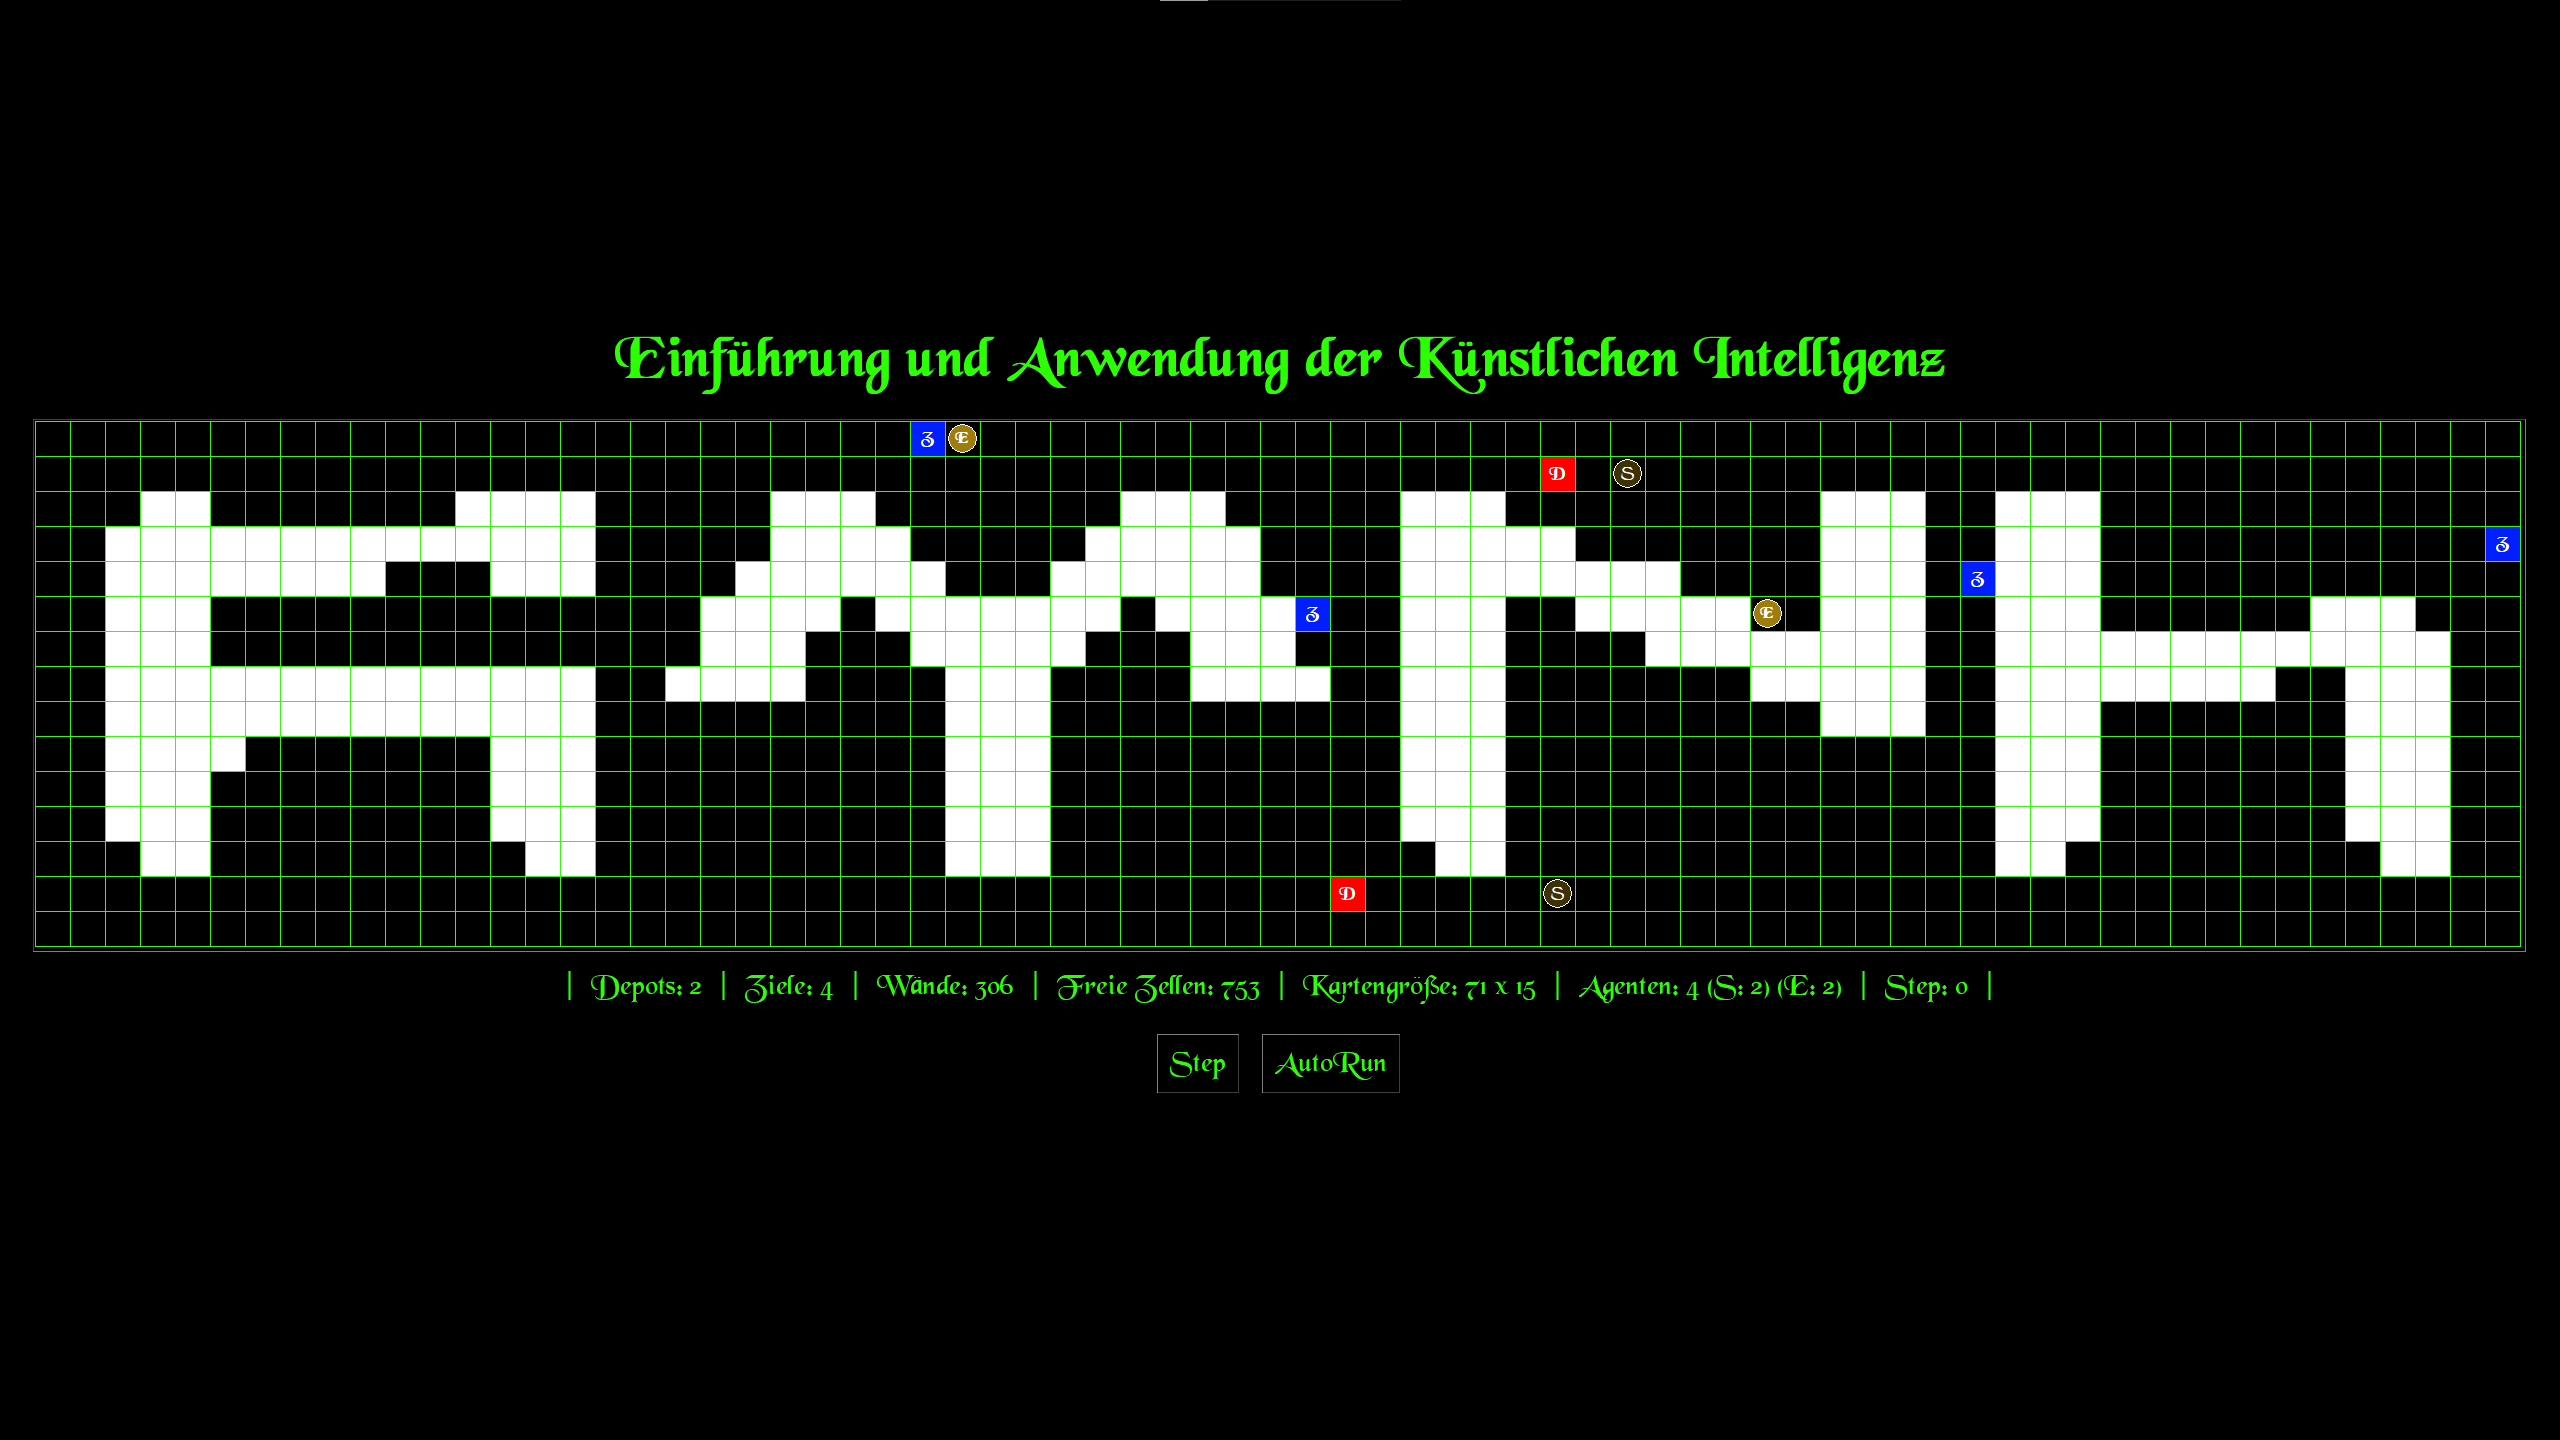
\includegraphics[width=1\textwidth]{asset/image/1C-GUI.png}
    \caption{Grafische Darstellung der Simulation im Initialzustand (\acs{S} = Standard, \acs{E} = Express)}
    \label{fig:simulation1c_gui_initial}
\end{figure}

Abbildung~\ref{fig:simulation1c_gui_step5} zeigt die \acs{GUI} nach fünf Simulationsschritten. Die Agenten haben sich entsprechend der zufälligen Richtungswahl über die Karte verteilt; die Positionen und der Batteriestand in der Agenten-Tabelle der Konsole spiegeln den Fortschritt wider.

\begin{figure}[H]
    \centering
    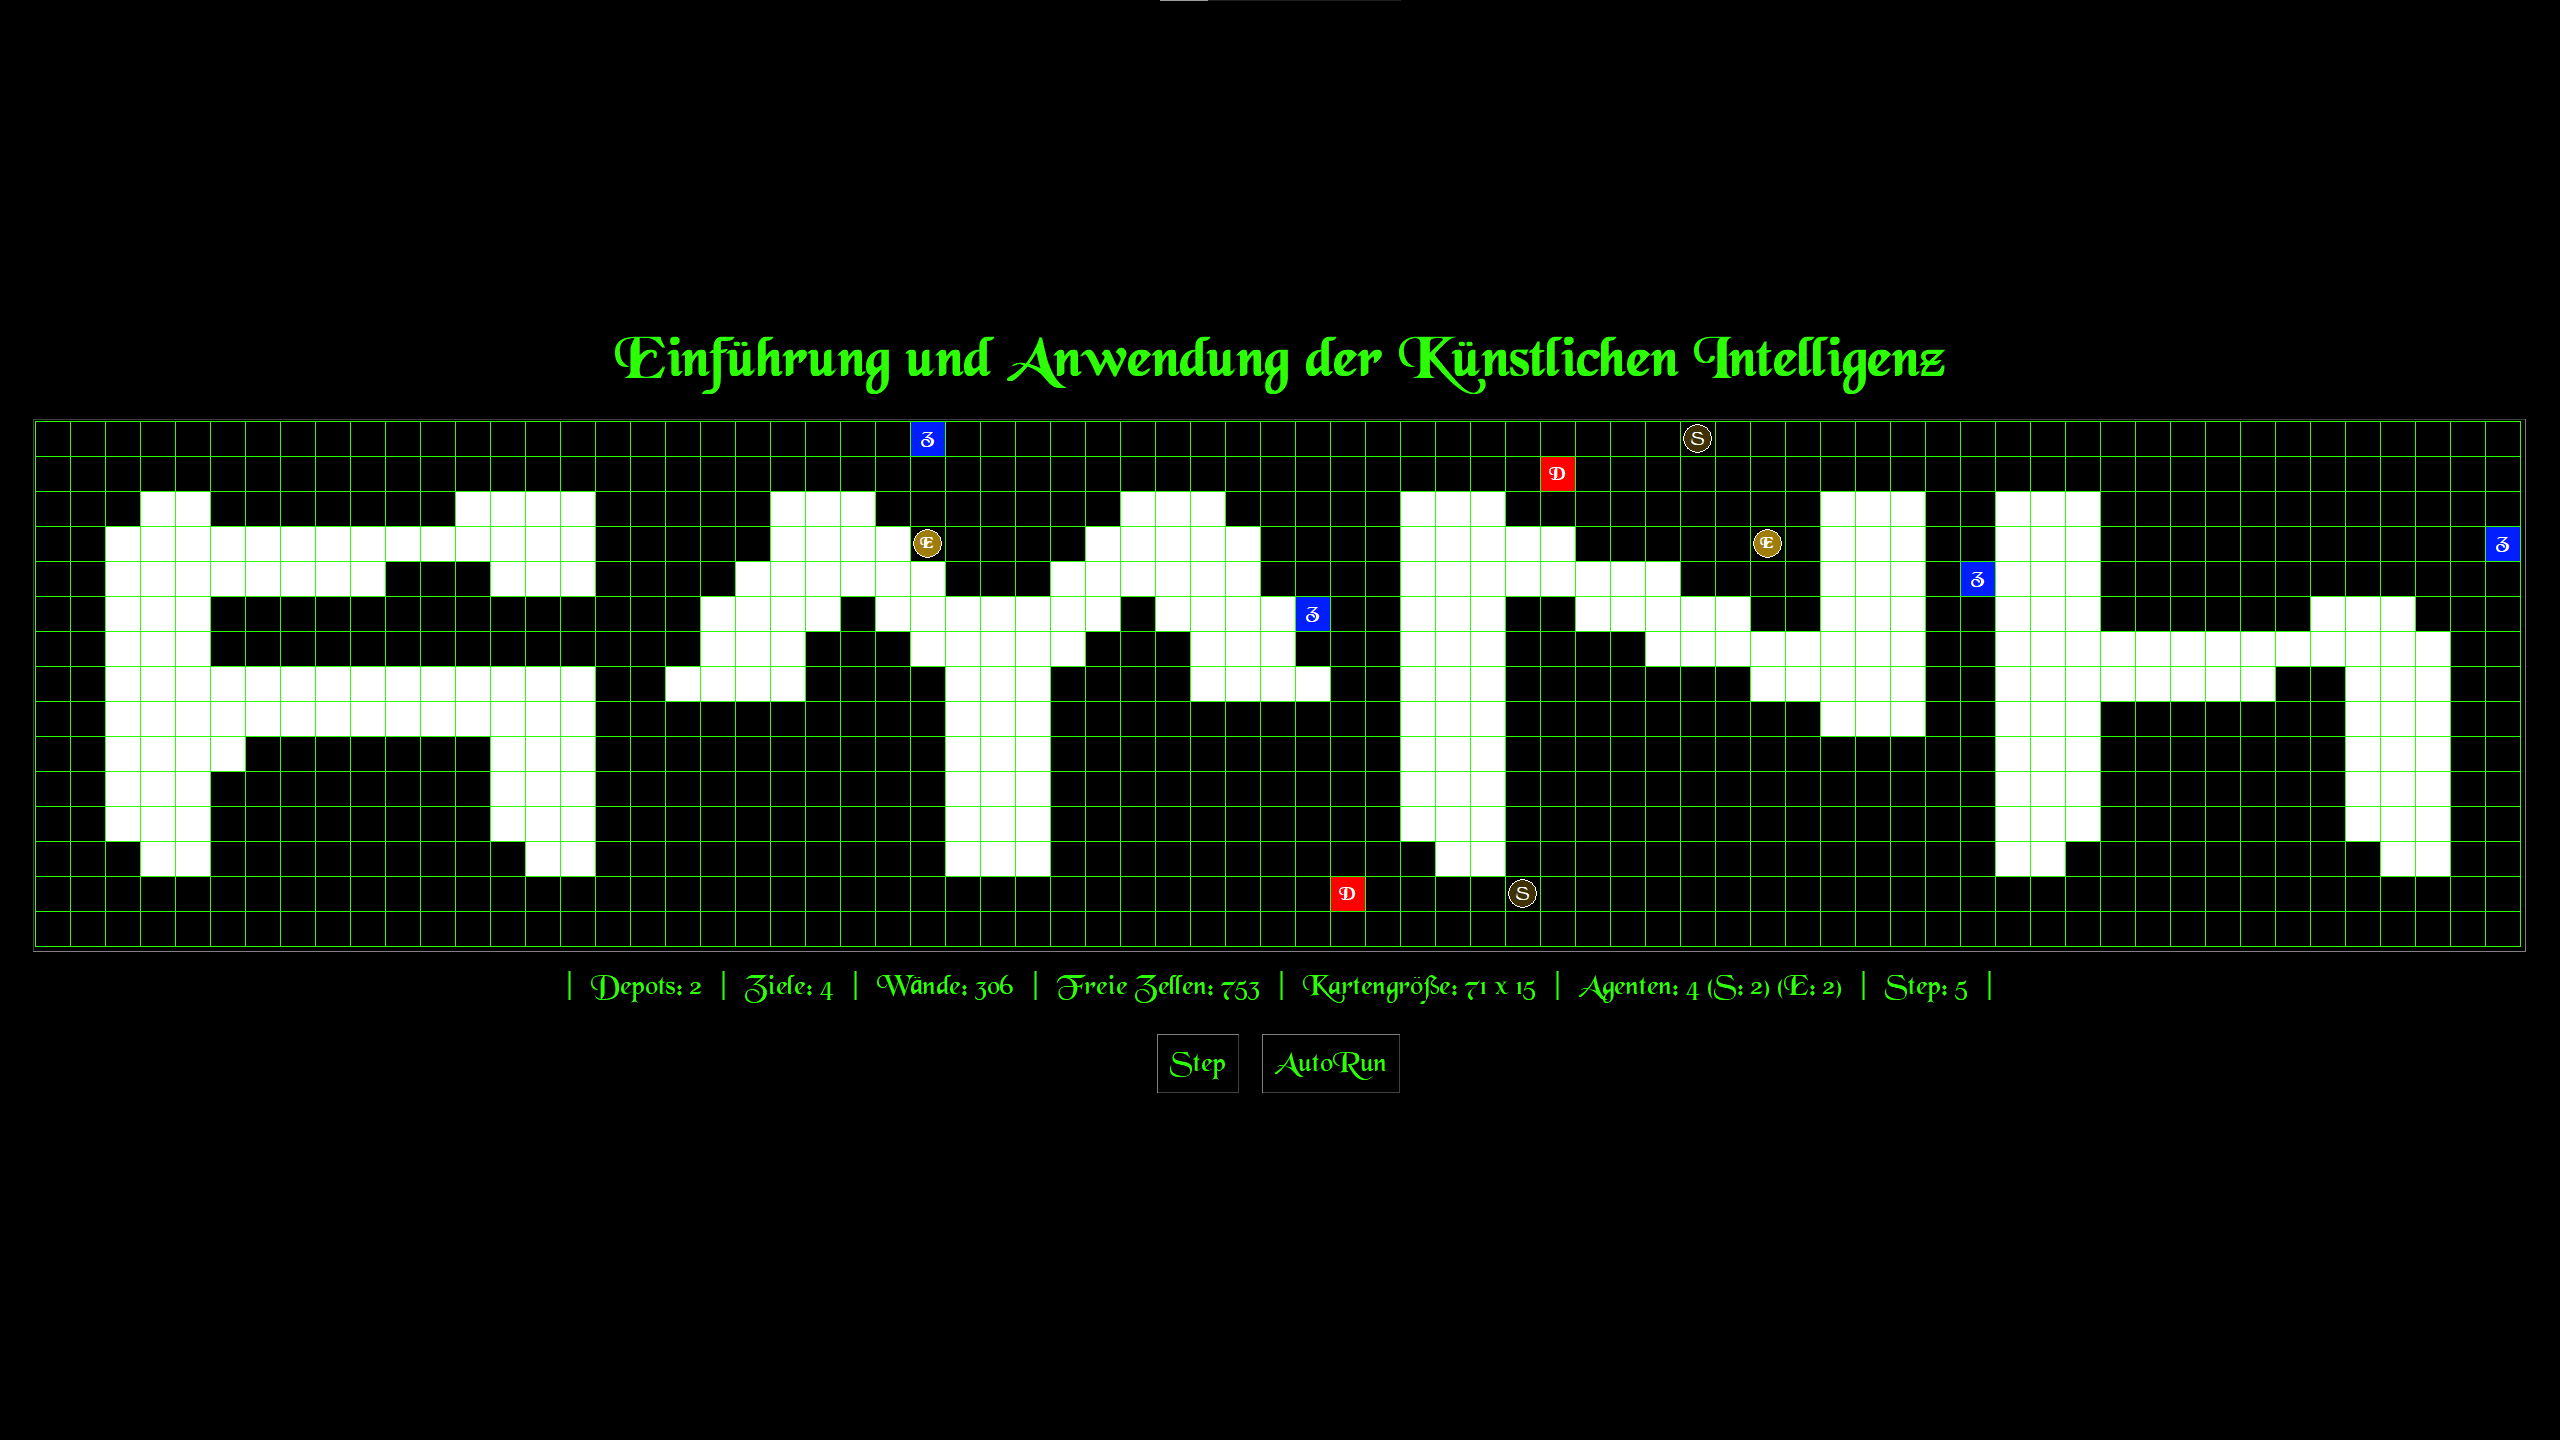
\includegraphics[width=1\textwidth]{asset/image/1C-GUI-II.png}
    \caption{Grafische Darstellung der Simulation nach fünf Simulationsschritten}
    \label{fig:simulation1c_gui_step5}
\end{figure}

Auf der Konsole wird zuerst der Initialzustand der Agenten (aus Aufgabe~1b) und anschließend die ersten fünf Schritt-Protokolle vollständig ausgegeben:

\lstinputlisting[
    style=console,
    caption={Terminal-Ausgabe: Initialzustand und fünf Simulationsschritte},
    label={lst:simulation_1c_terminal}
    firstline=31,
    lastline=75
]{asset/code/1C-terminal.tex}

Die Ausgabe zeigt:
\begin{itemize}
    \item Die Step-Überschrift wird mittig auf der konfigurierten Trennlinienlänge zentriert; die Zeilen davor und danach bilden die konfigurierten Trennzeichen (\texttt{TomaKingGUI\_LogSeparatorCharLine}).
    \item Ab dem ersten Schritt werden Nachrichten-Events in einem eigenen Block zwischen Step-Header und Agentenliste ausgegeben. Der Versand erfolgt alle \texttt{TomaKing1C\_MessageInterval}~=~5 Schritte durch die Methode \texttt{\_dispatch\_message}.
    \item Die Agentenzeilen verwenden dasselbe Spaltenformat wie in Aufgabe~1b \\ (\texttt{TomaKing1B\_LogColumnFormat}); der Fortschritt ist an Position und Batteriestand erkennbar.
    \item Die Express-Agenten (Speed~2) verbrauchen pro Schritt bis zu zwei Batterieeinheiten, sofern beide Bewegungen ausgeführt werden konnten. Bei blockierter Bewegung wird kein Verbrauch berechnet (\texttt{TomaKing1C\_BatteryStandstill}~=~0).
    \item Die Positionen sind zufällig, aber durch den Seed reproduzierbar -- der Zufallszahlengenerator wird mit \texttt{TomaKing1C\_Seed} initialisiert.
\end{itemize}

Die Anfangspositionen der Agenten und ihre Bewegung nach fünf Schritten sind in Tabelle~\ref{tab:simulation1c_movement} zusammengefasst.

\begin{table}[H]
    \centering
    \begin{tabular}{c l r r r}
        \toprule
        \textbf{Agent} & \textbf{Typ} & \textbf{Position (Step 0)} & \textbf{Position (Step 5)} & \textbf{Batterie (Step 5)} \\
        \midrule
        0 & Standard & (43, 13) & (42, 13) & 97/100 \\
        1 & Standard & (45, 1)  & (47, 0)  & 95/100 \\
        2 & Express  & (26, 0)  & (25, 3)  & 112/120 \\
        3 & Express  & (49, 5)  & (49, 3)  & 112/120 \\
        \bottomrule
    \end{tabular}
    \caption{Bewegung der Agenten nach fünf Simulationsschritten}
    \label{tab:simulation1c_movement}
\end{table}

Die Spalte \textit{Batterie (Step~5)} zeigt die Werte in der Form \textit{aktuell/Maximum}. Die Standard-Agenten haben in fünf Schritten zwischen 3 und 5 Batterieeinheiten verbraucht (abhängig davon, ob die zufällige Bewegung blockiert wurde); die Express-Agenten zwischen 5 und 8 Einheiten (Speed~2). Der Nachrichten-Austausch zwischen den Agenten ist an den Event-Blöcken in der Konsolenausgabe erkennbar (\texttt{[SEND]}~und~\texttt{[READ]}).

% ==============================================================================
% ================================= Aufgabe 1 =================================
% ==============================================================================